\chapter{Resultados de Simulação e Experimentais}

Neste capítulo são exibidos os resultados de simulação e experimentais. A simulação mostrada é de um rastreamento de trajetória no espaço operacional, pois é representativa do comportamento do sistema. Para experimentos com o manipulador TETIS foram feitos testes em varias etapas, em crescente nível de complexidade. Iniciando com uma análise da malha interna de controle, seguida de controle no espaço das juntas, controle proporcional de posição no espaço operacional, controle proporcional com feedforward e controle de força. As trajetórias utilizadas nos testes são definidas de antemão:

\textbf{Trajetória 1}
\begin{gather} \label{eq:traj1}
\bm{x_d} = \m{75 \sin(\omega_n t) + \sin (4 \omega_n t) + 500 \\ 57 \\ 75 \cos(\omega_n t) + \cos(4\omega_n t) -67 \\ \omega_n \sin(\omega_nt) }
\bm{\dot{x}_d} = \m{75\omega_n \cos(t\omega_n) + 300 \omega_n \cos(4t\omega_n) \\
0 \\
-75 \omega_n \sin(t \omega_n) - 300 \omega_n \sin(4t\omega_n) \\
\omega_n^2 \cos(t \omega_n)}
\end{gather}
onde $\omega_n = \pi/10$

\textbf{Trajetória 2}
\begin{align}
\bm{x_d} &= \m{ 
\ddfrac{100 \cos(t)}{\sin^2(t) + 1} + 500 \\
57 \\
\ddfrac{100\cos(t) \sin(t)}{\sin^2(t) + 1} -50 \\
0
} &&
\bm{\dot{x}_d} = \m{
\ddfrac{100\sin(t) (\sin^2(t) -3 )}{(\sin^2(t) + 1)^2} \\
0 \\
\ddfrac{-(300 \sin^2(t) - 100)}{(\sin^2(t) + 1)^2} \\
0}
\end{align}

\section{Simulação}
Utilizando a Robotics Toolbox \citep{petercorke} para MATLAB\circledR, foram feitas simulações para o controle cinemático utilizando controle proporcional com feedforward e a trejetória 1 \eqref{eq:traj1} como referência.

\begin{figure}[H]
\centering
  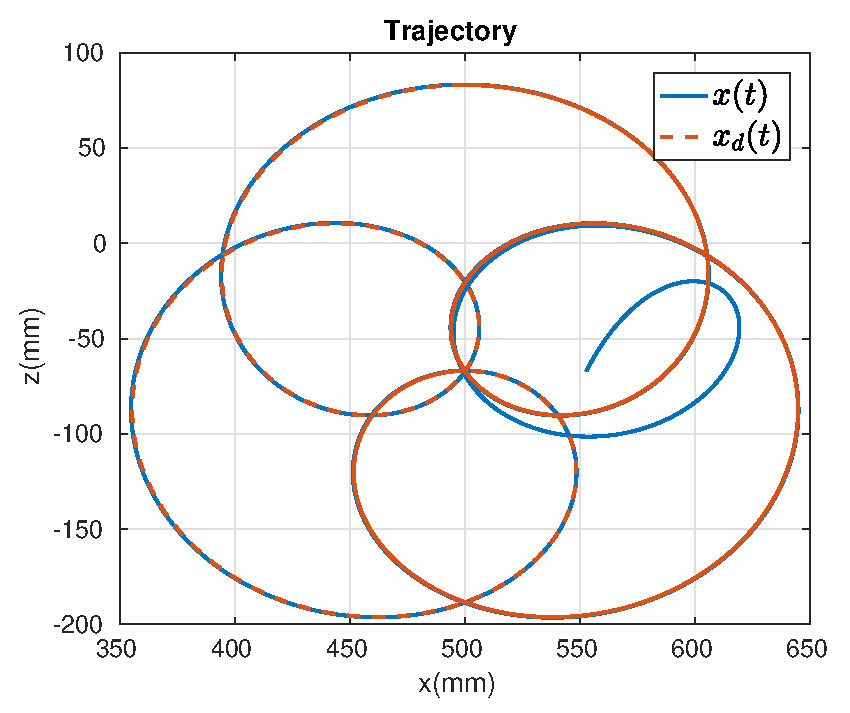
\includegraphics[width=0.5\linewidth]{./img/simul_delay_zoh1/traj.eps}
  \caption{Simulação: Trajetória 1 no plano x-z}
  \label{fig:sub1}
\end{figure}%

\begin{figure}[H]
\centering
\begin{subfigure}{.5\textwidth}
  \centering
  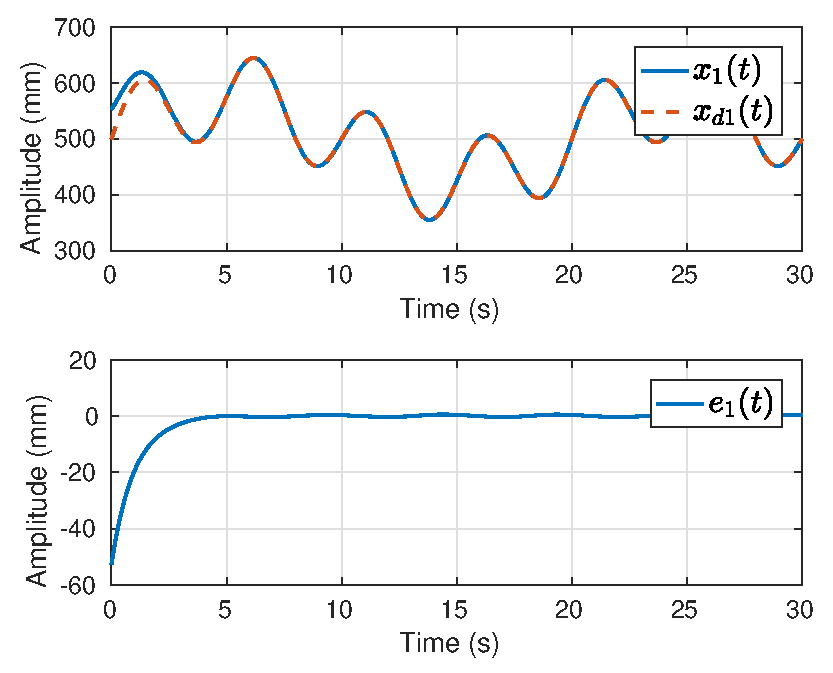
\includegraphics[width=\linewidth]{./img/simul_delay_zoh1/x1.eps}
  \caption{$x$}
  \label{fig:sub1}
\end{subfigure}%
\begin{subfigure}{.5\textwidth}
  \centering
  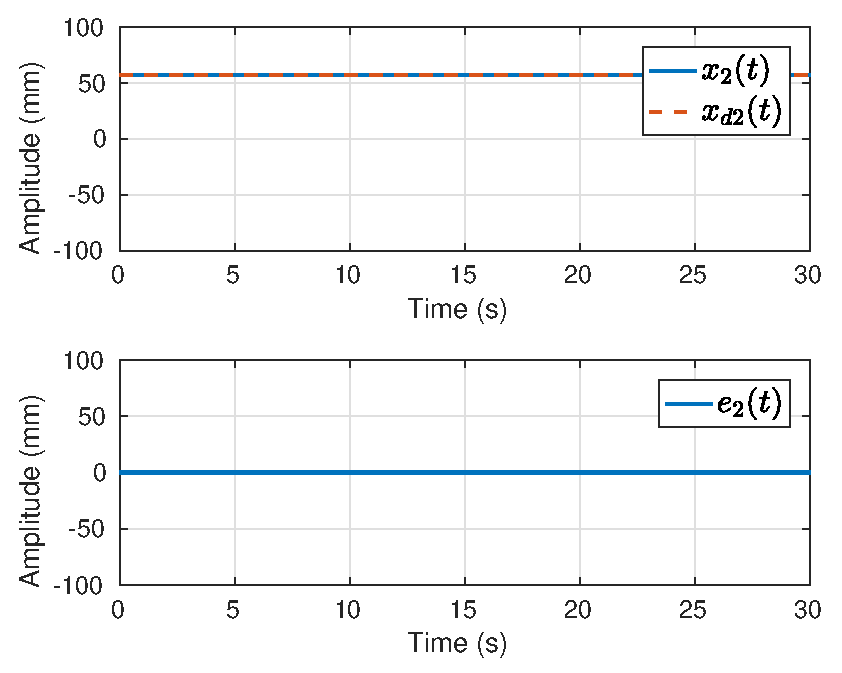
\includegraphics[width=\linewidth]{./img/simul_delay_zoh1/x2.eps}
  \caption{$y$}
  \label{fig:sub2}
\end{subfigure}
\begin{subfigure}{.5\textwidth}
  \centering
  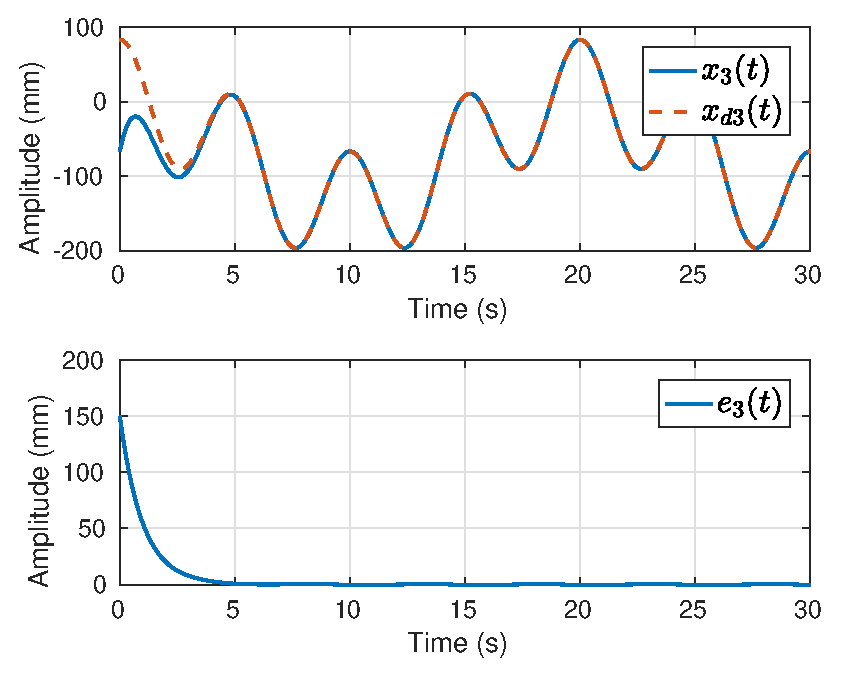
\includegraphics[width=\linewidth]{./img/simul_delay_zoh1/x3.eps}
  \caption{$z$}
  \label{fig:sub1}
\end{subfigure}%
\begin{subfigure}{.5\textwidth}
  \centering
  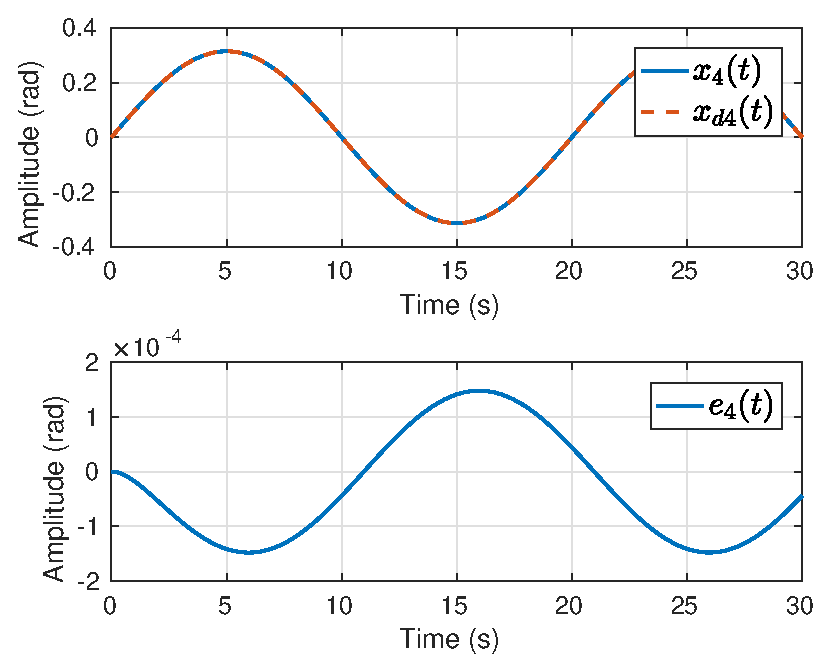
\includegraphics[width=\linewidth]{./img/simul_delay_zoh1/x4.eps}
  \caption{$\phi$}
  \label{fig:sub2}
\end{subfigure}
\caption{Simulação: Rastreamento da trajetória 1 para $\bm{K}_t = \bm{I}$}
\label{fig:test}
\end{figure}

\begin{figure}[H]
\centering
\begin{subfigure}{.5\textwidth}
  \centering
  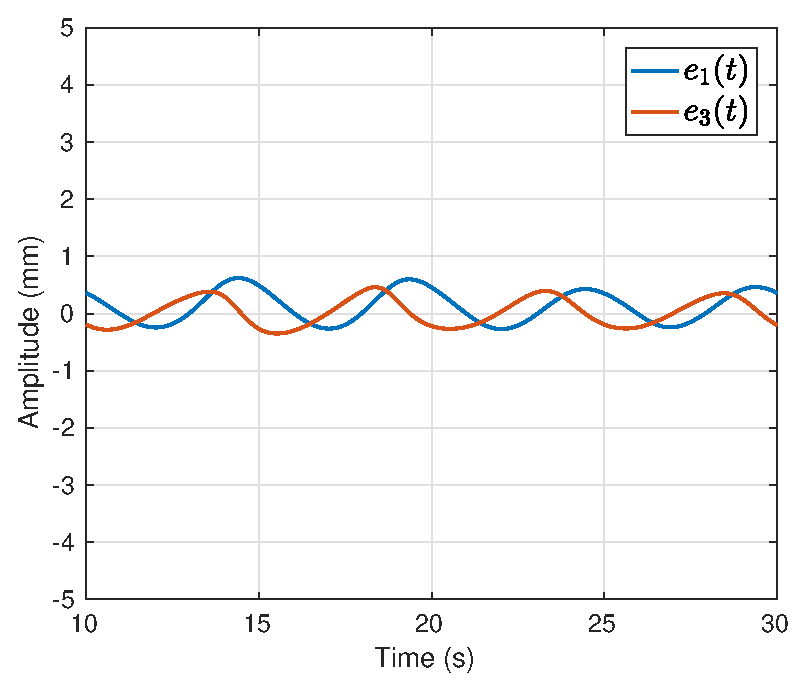
\includegraphics[width=\linewidth]{./img/simul_delay_zoh1/error.eps}
  \caption{$e_1$ e $e_3$}
  \label{fig:sub1}
\end{subfigure}%
\begin{subfigure}{.5\textwidth}
  \centering
  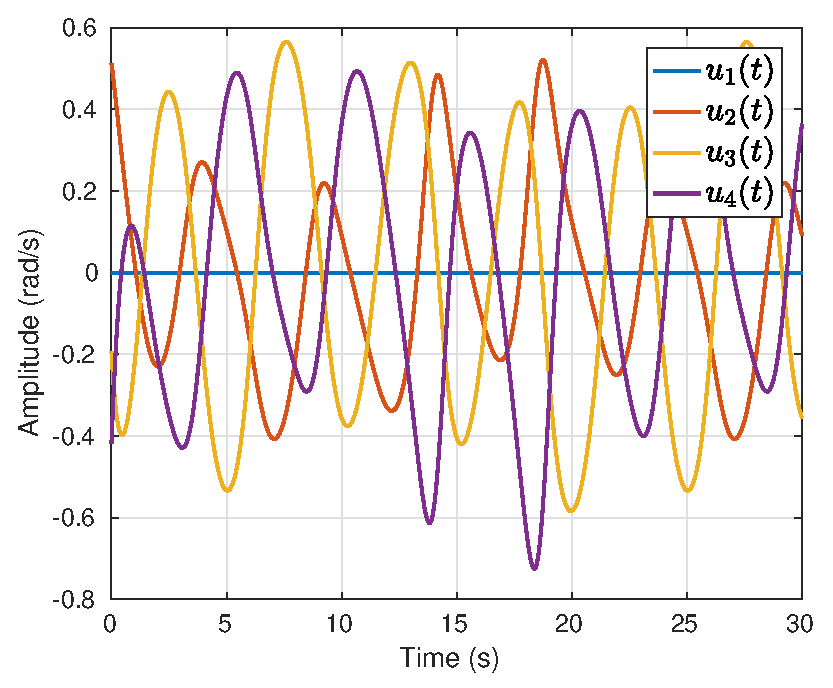
\includegraphics[width=\linewidth]{./img/simul_delay_zoh1/u.eps}
  \caption{$\bm{u}(t)$}
  \label{fig:sub2}
\end{subfigure}
\caption{Simulação: Destaque para o erro $e_1$ e $e_3$ com $\bm{K}_t = \bm{I}$}
\label{fig:erro_traj}
\end{figure}


\section{Análise da Malha de Controle a nível de Juntas}
Para verificar se de fato são válidas as premissas assumidas na seção \ref{sec:controle_cinematico} para aplicação de uma estratégia de controle cinemático foi levantada para cada uma das juntas a resposta a uma onda quadrada tal que:
\[ u = A \sgn(\sin( 2\pi t/f)) \]
onde o período $T = 1/f = 1s$ e a amplitude $A = 0.5 rad/s$

\newlength{\imageheight}
\begin{figure}[H]
  \centering
  	\settoheight{\imageheight}{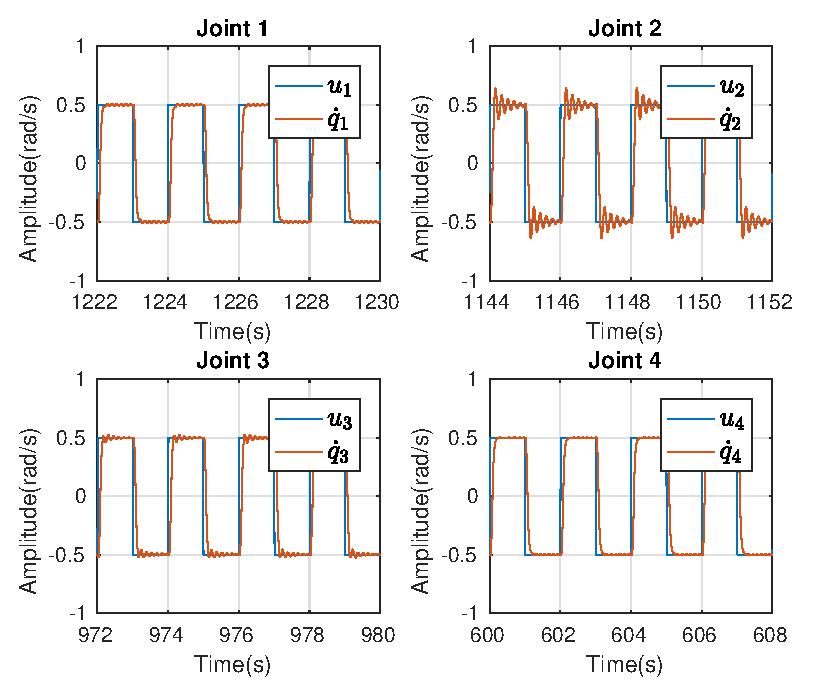
\includegraphics{./img/internal_loop}}
    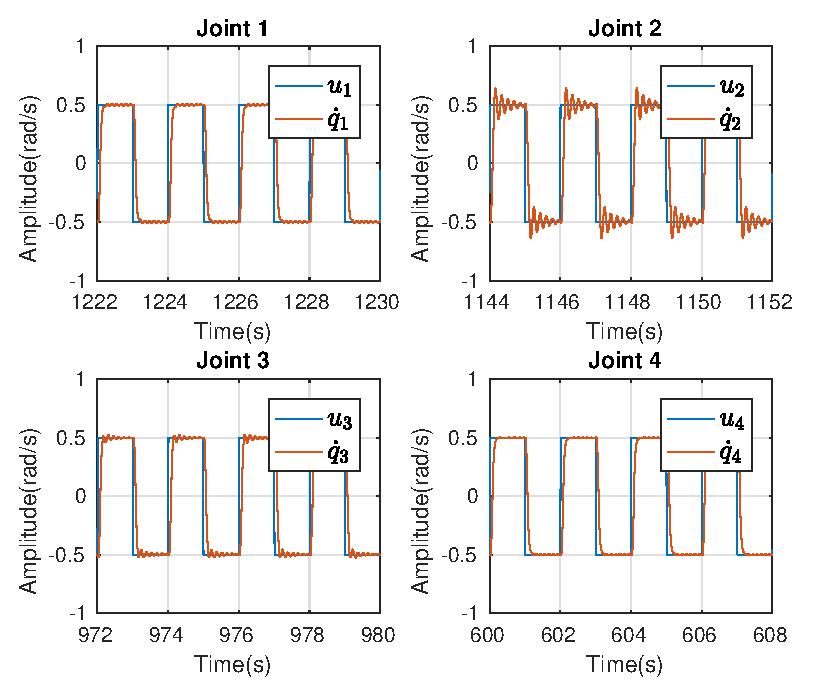
\includegraphics[width=\textwidth, clip=true, trim = 0 0.5\imageheight 0 0 0 mm]{./img/internal_loop}
  \caption{Resposta de velocidade das juntas 1 e 2}
\end{figure}

\begin{figure}[H]
  \centering
  	\settoheight{\imageheight}{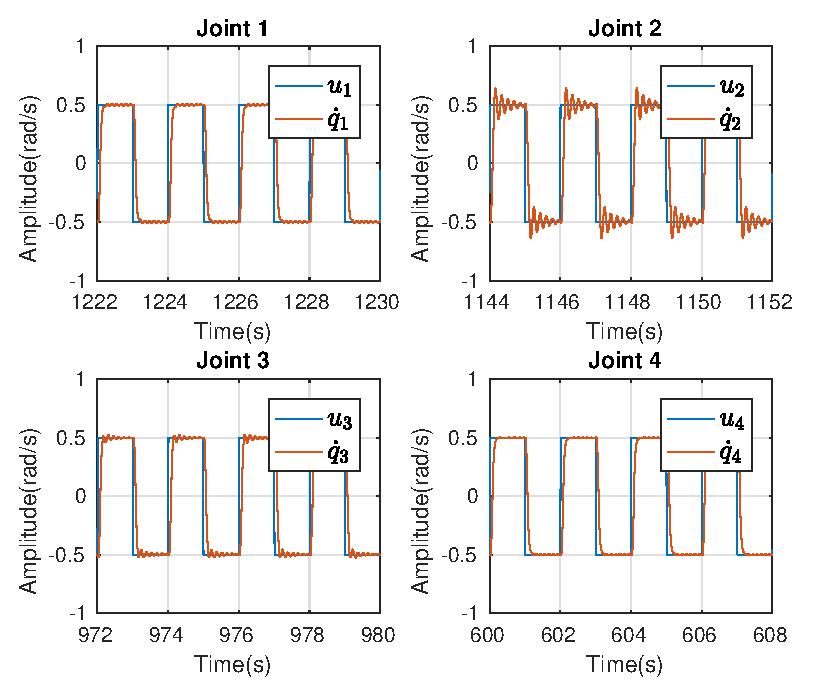
\includegraphics{./img/internal_loop}}
    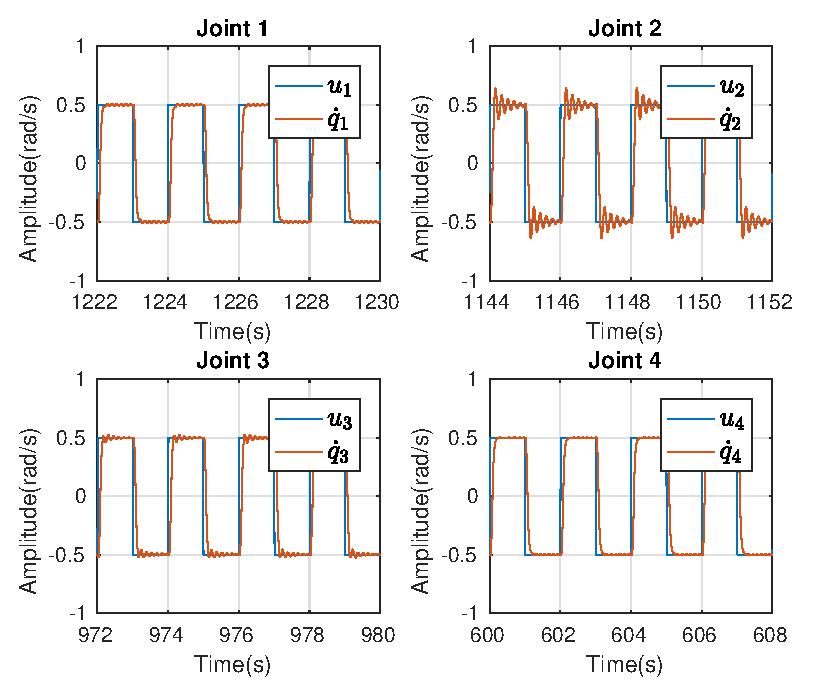
\includegraphics[width=\textwidth, clip=true, trim = 0 0 0 0.5\imageheight 0 mm]{./img/internal_loop}
  \caption{Resposta de velocidade das juntas 3 e 4}
\end{figure}

Observa-se que para as juntas 1, 3 e 4 a resposta é de primeira ordem e que são capazes de reproduzir com precisão os comandos de velocidade. A junta 2 observa-se que existe uma dinâmica. Isso se deve ao fato de a junta 2 necessitar de um torque maior para vencer a ação da força gravitacional. O controle cinemático produz resultados satisfatórios somente quando não são necessários movimentos muito rápidos ou acelerações muito grandes.


%mais suscetível a ação da força gravitacional, devido a uma maior dist
	

\section{Controle de Posição no Espaço das Juntas}

Neste experimento foi testado controle de posição no espaço das juntas, conforme definido em \ref{sec:position_joint}. Partindo da posição $\bm{q} =[ 0 \;\; -\pi/2 \;\; 0 \;\; 0]^T$, deseja-se atingir a posição $\bm{q} =[ 0 \;\; -\pi/4 \;\; \pi/2  \;\; -\pi/4]^T$. Foi utilizado um ganho $\bm{K}_j = \bm{I}$.

Os resultados foram conforme esperados, levando o erro assintoticamente a zero em todas as juntas.

\begin{figure}[H]
\centering
\begin{subfigure}{.5\textwidth}
  \centering
  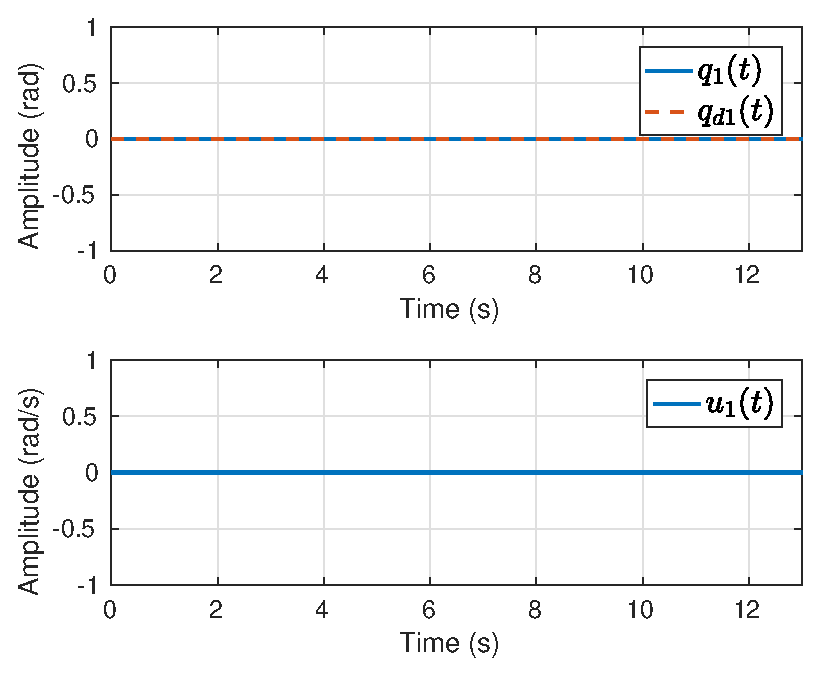
\includegraphics[width=\linewidth]{./img/joint_test1/q1.eps}
  \caption{Junta 1}
  \label{fig:sub1}
\end{subfigure}%
\begin{subfigure}{.5\textwidth}
  \centering
  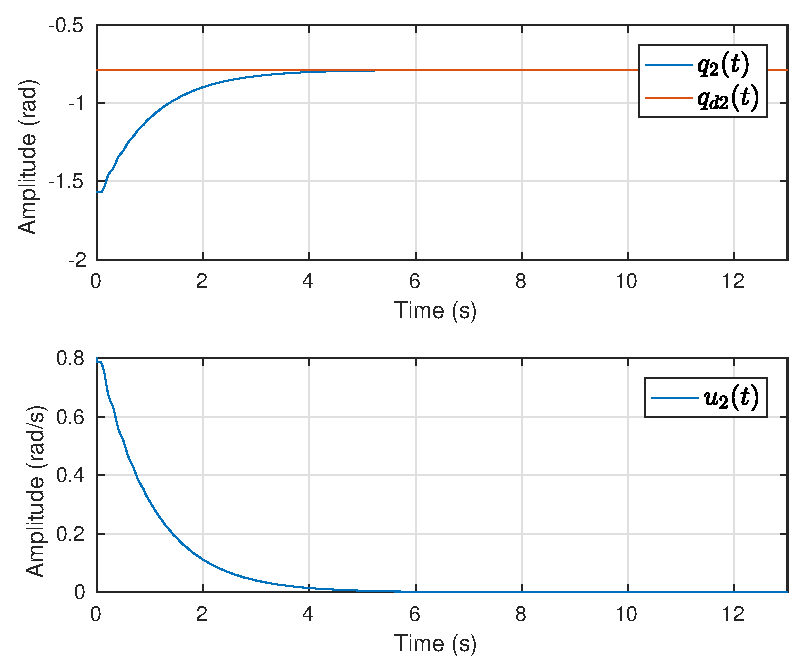
\includegraphics[width=\linewidth]{./img/joint_test1/q2.eps}
  \caption{Junta 2}
  \label{fig:sub2}
\end{subfigure}
\begin{subfigure}{.5\textwidth}
  \centering
  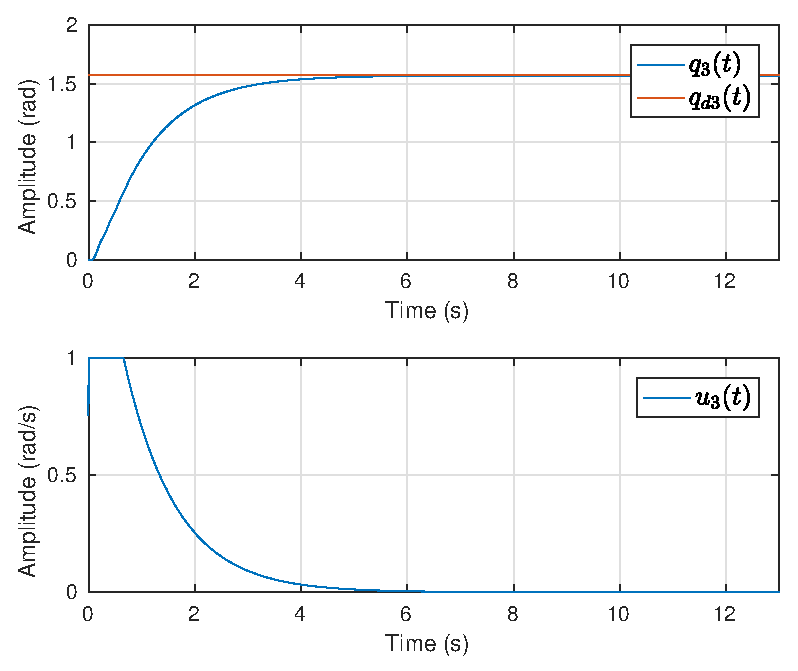
\includegraphics[width=\linewidth]{./img/joint_test1/q3.eps}
  \caption{Junta 3}
  \label{fig:sub1}
\end{subfigure}%
\begin{subfigure}{.5\textwidth}
  \centering
  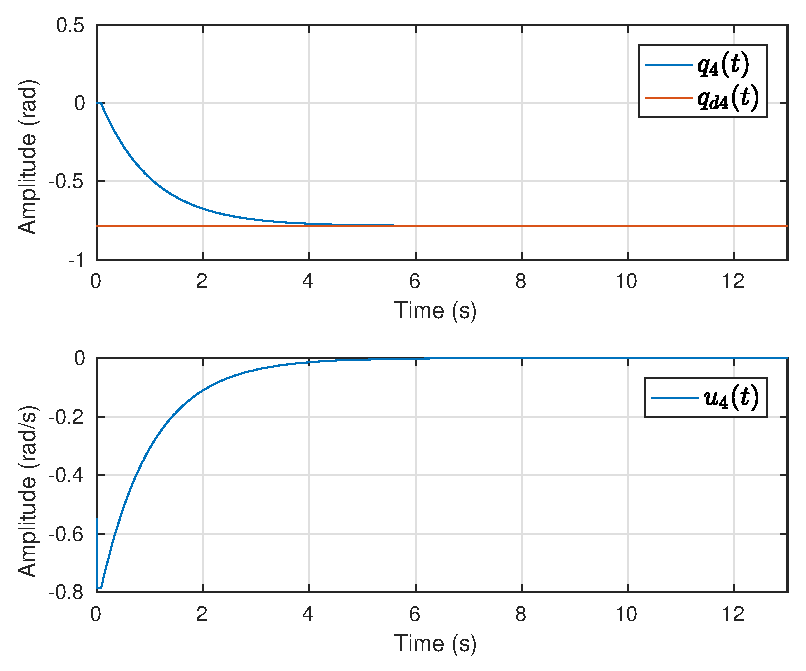
\includegraphics[width=\linewidth]{./img/joint_test1/q4.eps}
  \caption{Junta 4}
  \label{fig:sub2}
\end{subfigure}
\caption{Controle de Posição no Espaço das Juntas: Resultado experimental}
\label{fig:test}
\end{figure}


\section{Controle de Posição no Espaço Operacional}

Nesta seção, demonstra-se o controle no espaço operacional. Utilizando a estratégia de controle proporcional conforme definido na seção \ref{sec:pos_operacional}. 

\subsection{Experimento 1}

Neste experimento a posição inicial é $\bm{x} =[ 552.62 \; 57 \; -67.17 \; 0]^T$ e deseja-se alcançar $\bm{x}_d =[ 500 \; -50 \; -150 \; 0.5235]^T$. Utiliza-se um ganho $\bm{K}_p = \bm{I}$. A figura \ref{fig:oper_space_exp1} mostra que para o resultado para o problema de \textit{set-point}, o sistema foi capaz de rastrear assintoticamente um sinal de referência constante. 

\begin{figure}[H]
\centering
\begin{subfigure}{.5\textwidth}
  \centering
  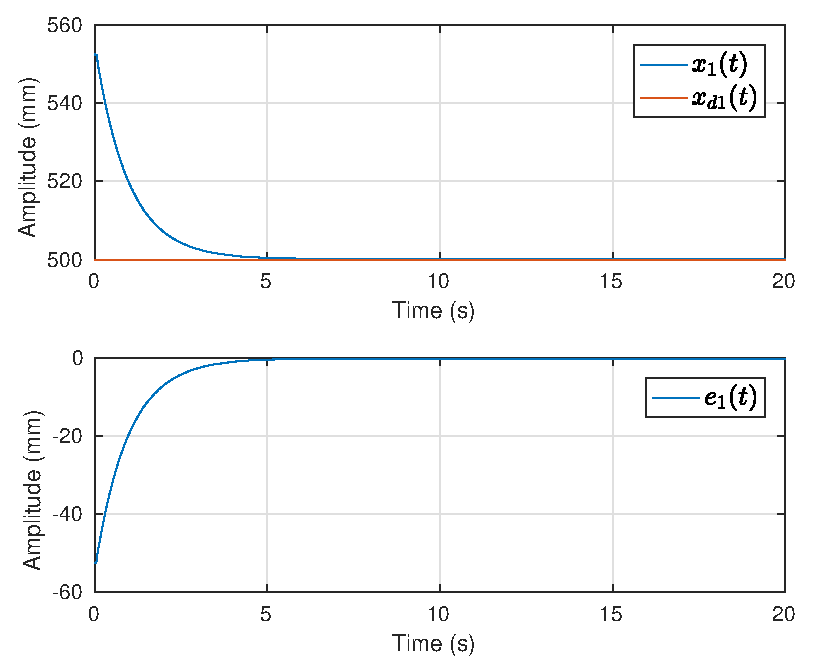
\includegraphics[width=\linewidth]{./img/position1/x1.eps}
  \caption{$x$}
  \label{fig:oper_space_exp1_x1}
\end{subfigure}%
\begin{subfigure}{.5\textwidth}
  \centering
  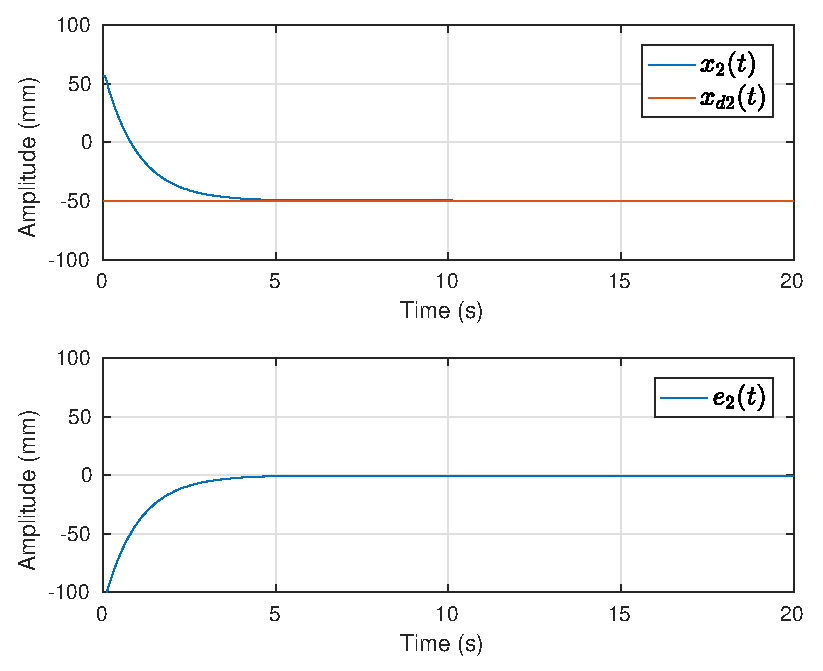
\includegraphics[width=\linewidth]{./img/position1/x2.eps}
  \caption{$y$}
  \label{fig:oper_space_exp1_x2}
\end{subfigure}
\begin{subfigure}{.5\textwidth}
  \centering
  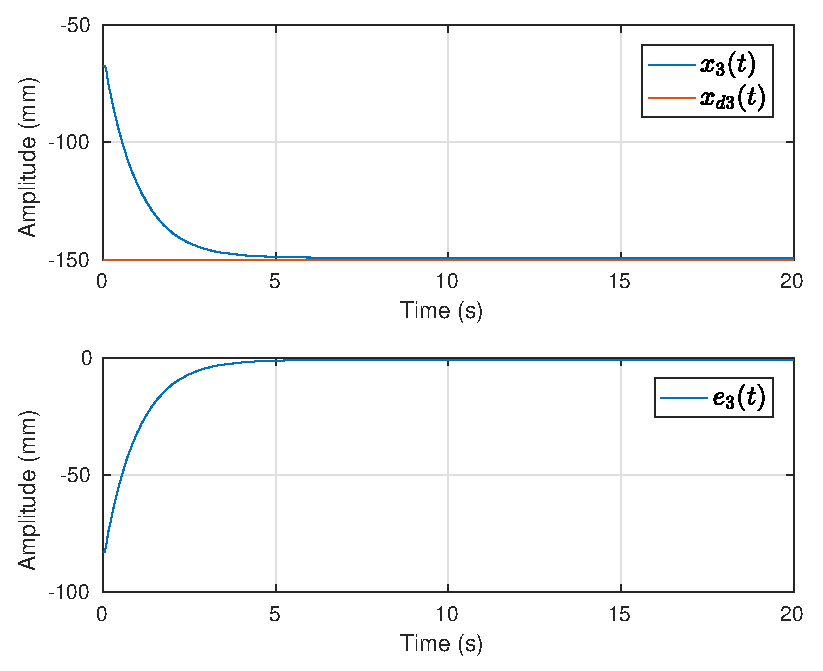
\includegraphics[width=\linewidth]{./img/position1/x3.eps}
  \caption{$z$}
  \label{fig:oper_space_exp1_x3}
\end{subfigure}%
\begin{subfigure}{.5\textwidth}
  \centering
  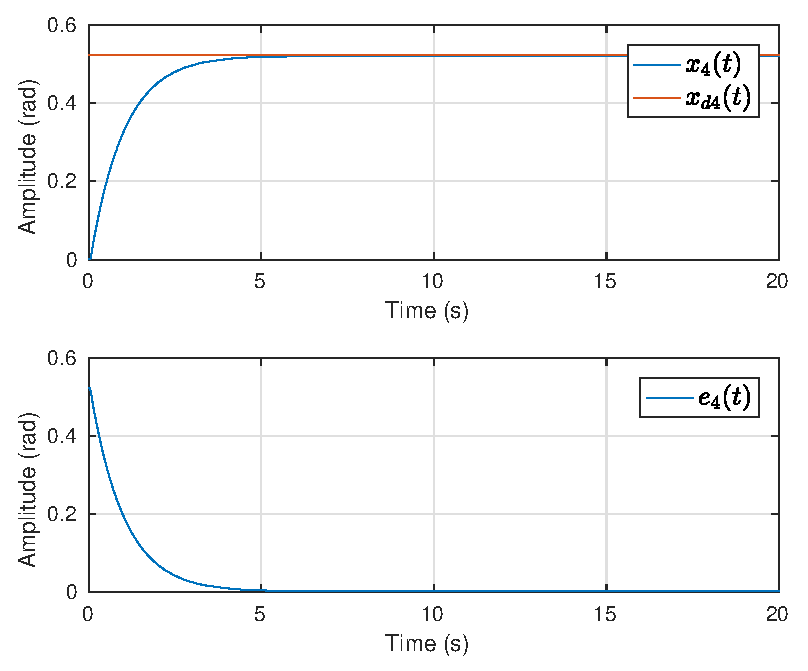
\includegraphics[width=\linewidth]{./img/position1/x4.eps}
  \caption{$\phi$}
  \label{fig:oper_space_exp1_x4}
\end{subfigure}
\caption{Controle de Posição no Espaço Operacional: Experimento 1}
\label{fig:oper_space_exp1}
\end{figure}

\subsection{Experimento 2}

Neste experimento, o objetivo é testar a alteração da orientação, mantendo a posição constante. A posição inicial é $\bm{x} =[ 550 \; 57 \; -100 \; 0]^T$. O gráfico \ref{fig:pos_exp2_phi} a orientação é alterada para $60^o$, ou seja $\bm{x_d} =[ 550 \; 57 \; -100 \; 1.0472]^T$. Em seguida, a orientação é alterada para $-60^o$, ou seja $\bm{x_d} =[ 550 \; 57 \; -100 \; -1.0472]^T$. 

Nas figuras \ref{fig:oper_space_exp2_x1} e \ref{fig:oper_space_exp2_x3} é possível identificar que a mudança de orientação gerou distúrbios nas dimensões $x$ e $z$. No entanto, os distúrbios foram rejeitados assintoticamente.

\begin{figure}[H]
\centering
\begin{subfigure}{.5\textwidth}
  \centering
  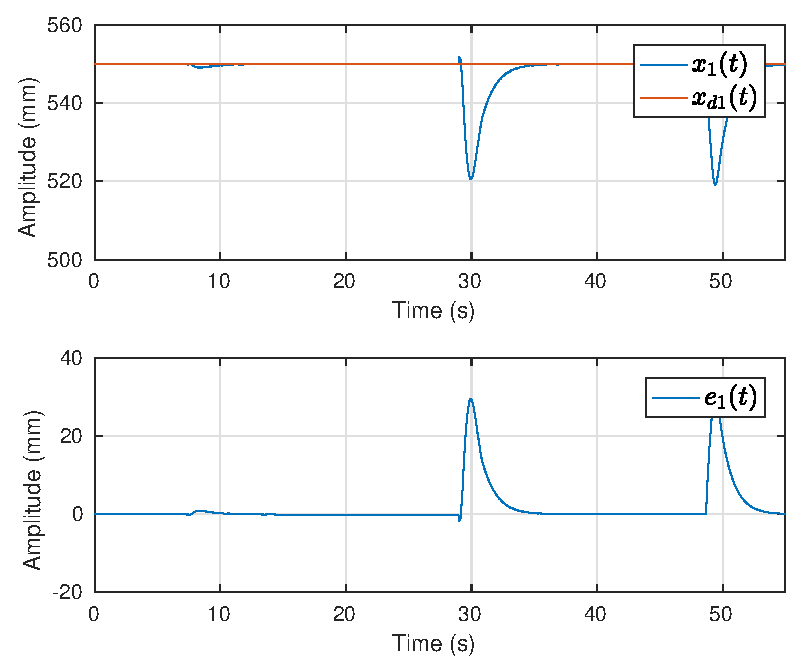
\includegraphics[width=\linewidth]{./img/position2/x1.eps}
  \caption{$x$}
  \label{fig:oper_space_exp2_x1}
\end{subfigure}%
\begin{subfigure}{.5\textwidth}
  \centering
  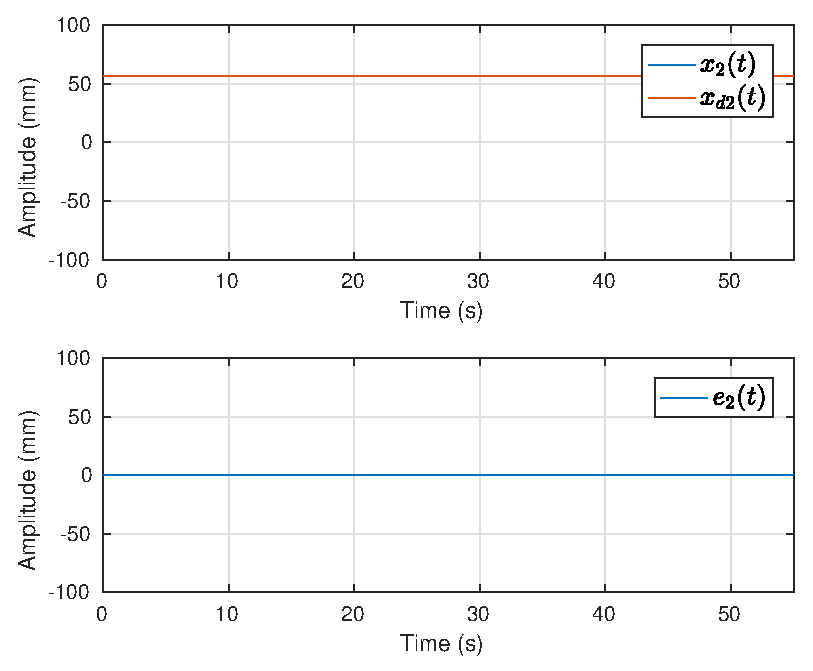
\includegraphics[width=\linewidth]{./img/position2/x2.eps}
  \caption{$y$}
  \label{fig:oper_space_exp2_x2}
\end{subfigure}
\begin{subfigure}{.5\textwidth}
  \centering
  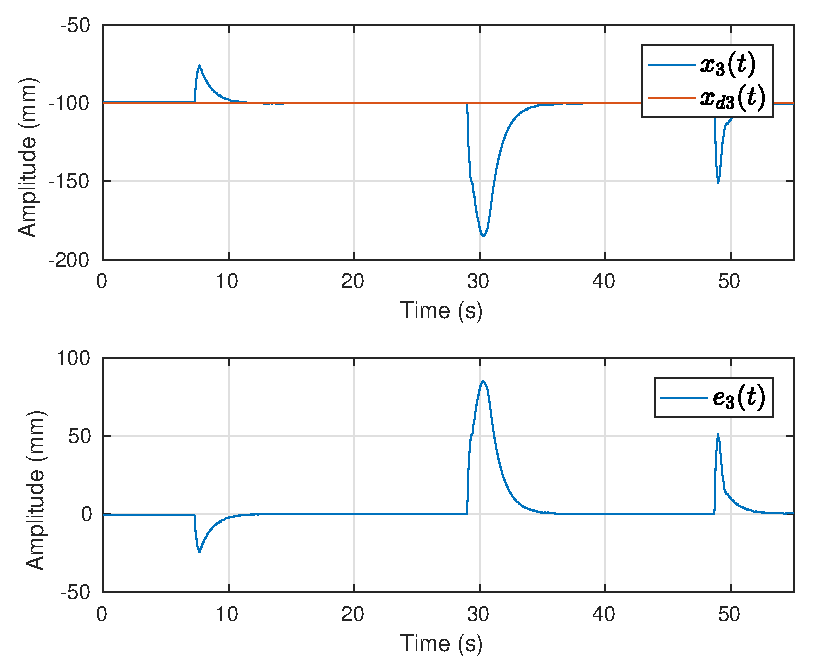
\includegraphics[width=\linewidth]{./img/position2/x3.eps}
  \caption{$z$}
  \label{fig:oper_space_exp2_x3}
\end{subfigure}%
\begin{subfigure}{.5\textwidth}
  \centering
  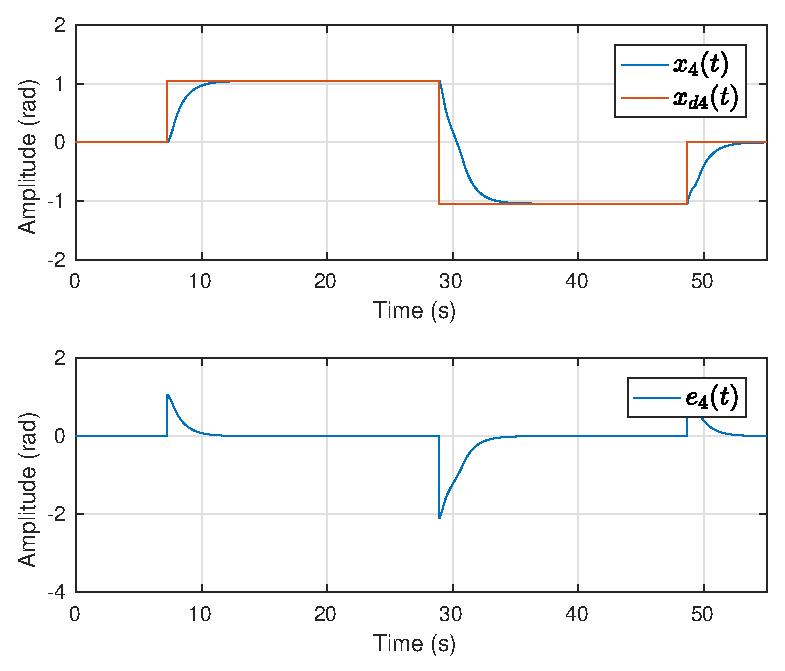
\includegraphics[width=\linewidth]{./img/position2/x4.eps}
  \caption{$\phi$}
  \label{fig:pos_exp2_phi}
\end{subfigure}
\caption{Controle de Posição no Espaço Operacional: Experimento 2}
\label{fig:oper_space_exp2}
\end{figure}

\section{Rastreamento de Trajetória}

Nesta seção são exibidos os resultados experimentais para o rastreamento das duas trajetórias definidas em \eqref{eq:traj1} e \eqref{eq:traj2}. Utiliza-se uma estratégia de controle proporcional com feedforward, conforme definido em \ref{sec:pplusf}. 

\subsection{Trajetória 1}

\subsubsection{Ganho $\bm{K}_t = \bm{I}$}

\begin{figure}[H]
\centering
  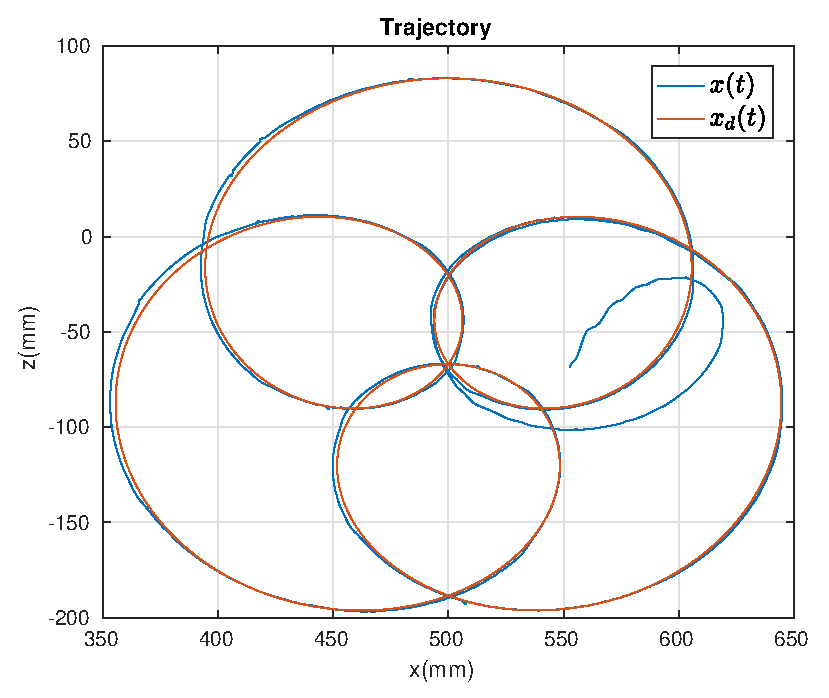
\includegraphics[width=0.5\linewidth]{./img/traj_1_k1/traj.eps}
  \caption{Trajetória 1 no plano x-z: Resultados experimentais com $\bm{K}_t = \bm{I}$}
  \label{fig:sub1}
\end{figure}%

\begin{figure}[H]
\centering
\begin{subfigure}{.5\textwidth}
  \centering
  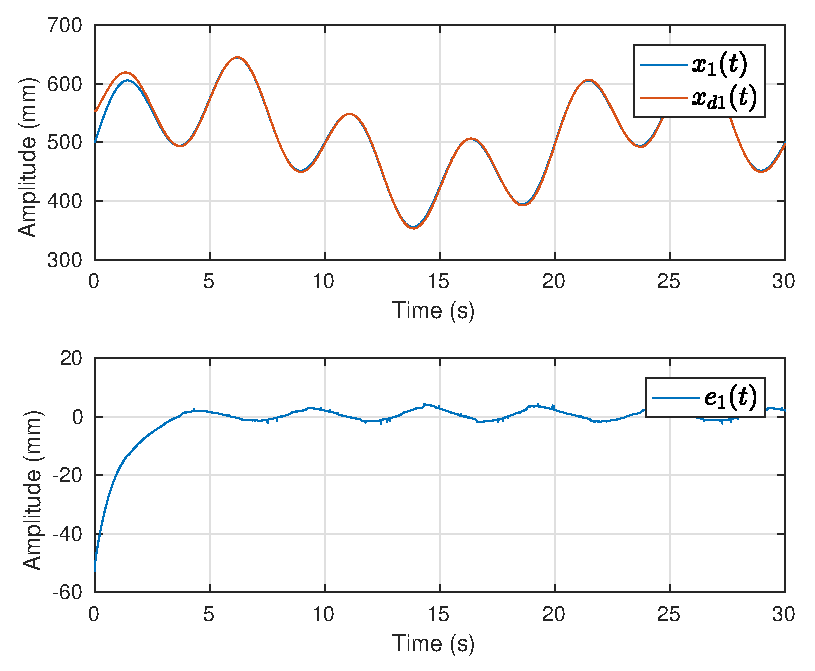
\includegraphics[width=\linewidth]{./img/traj_1_k1/x1.eps}
  \caption{$x_1$}
  \label{fig:sub1}
\end{subfigure}%
\begin{subfigure}{.5\textwidth}
  \centering
  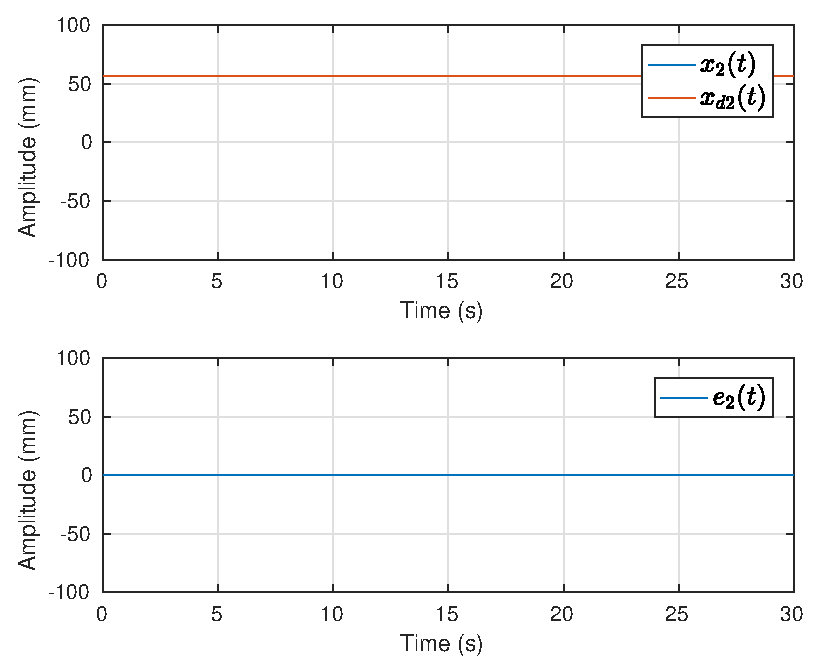
\includegraphics[width=\linewidth]{./img/traj_1_k1/x2.eps}
  \caption{$x_2$}
  \label{fig:sub2}
\end{subfigure}
\begin{subfigure}{.5\textwidth}
  \centering
  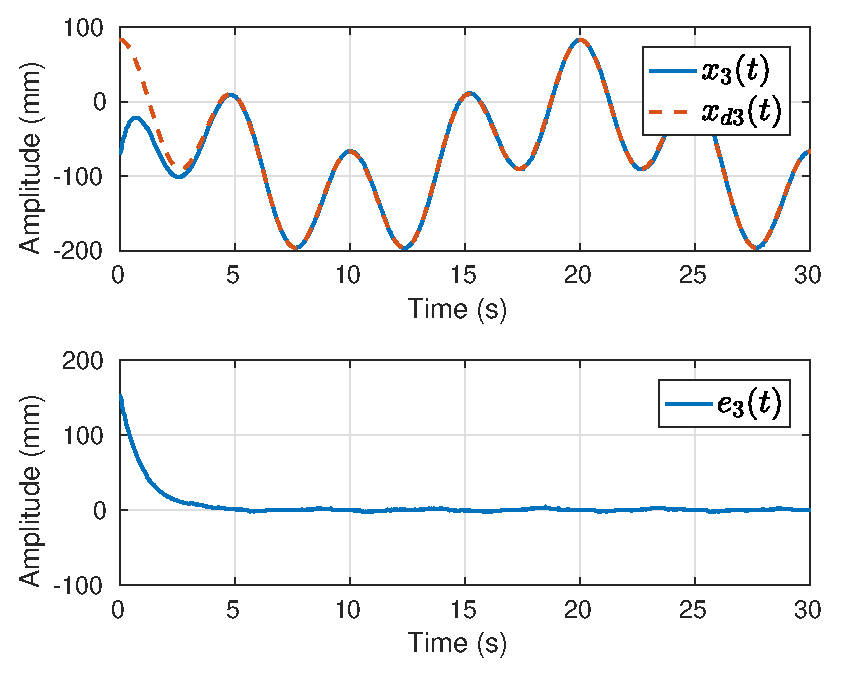
\includegraphics[width=\linewidth]{./img/traj_1_k1/x3.eps}
  \caption{$x_3$}
  \label{fig:sub1}
\end{subfigure}%
\begin{subfigure}{.5\textwidth}
  \centering
  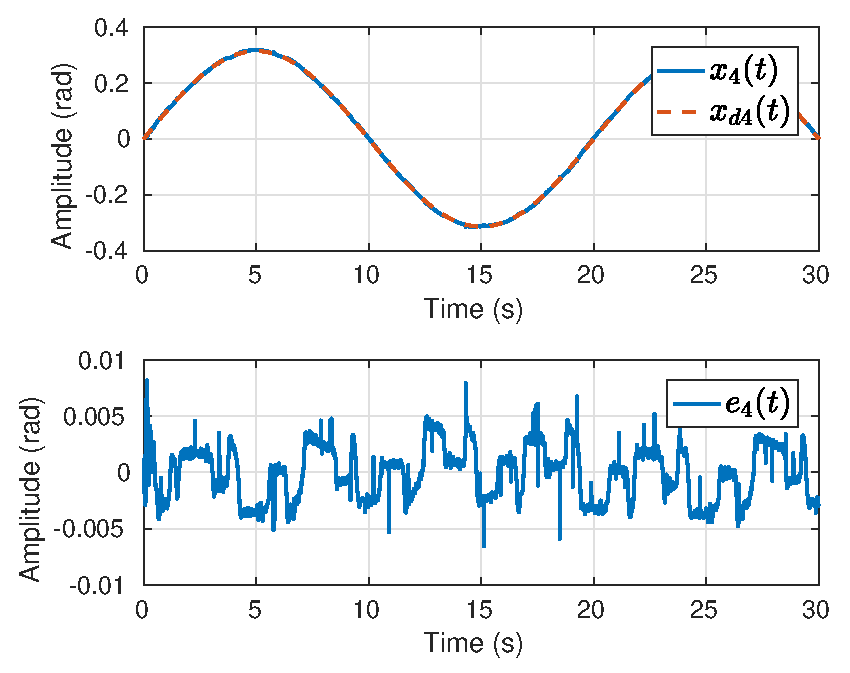
\includegraphics[width=\linewidth]{./img/traj_1_k1/x4.eps}
  \caption{$x_4$}
  \label{fig:sub2}
\end{subfigure}
\caption{Rastreamento da trajetória 1 para $\bm{K}_t = \bm{I}$: Resultados experimentais}
\label{fig:test}
\end{figure}

\begin{figure}[H]
\centering
\begin{subfigure}{.5\textwidth}
  \centering
  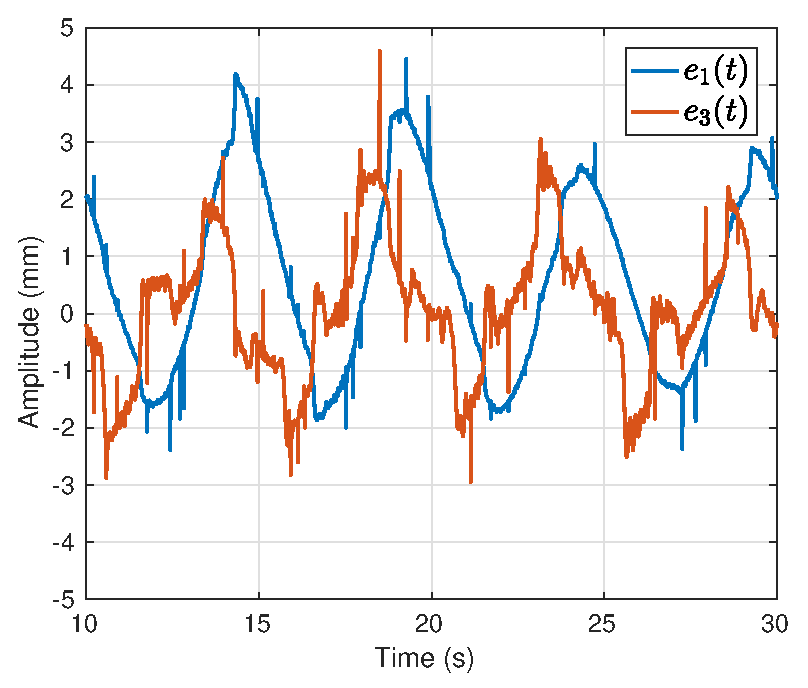
\includegraphics[width=\linewidth]{./img/traj_1_k1/error.eps}
  \caption{$e_1$ e $e_3$}
  \label{fig:sub1}
\end{subfigure}%
\begin{subfigure}{.5\textwidth}
  \centering
  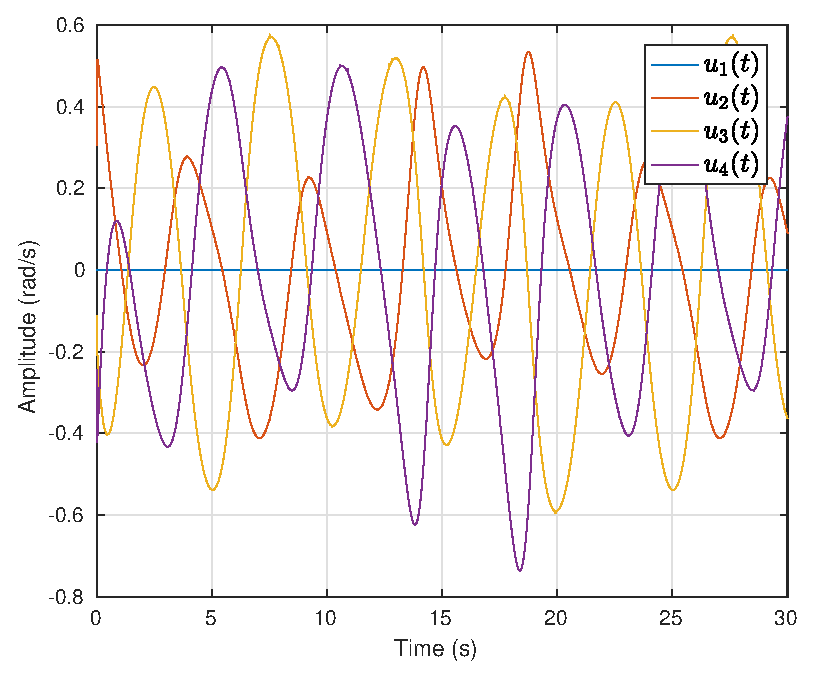
\includegraphics[width=\linewidth]{./img/traj_1_k1/u.eps}
  \caption{$\bm{u}(t)$}
  \label{fig:sub2}
\end{subfigure}
\caption{Trajetória 1, destaque para o erro $e_1$ e $e_3$ com $\bm{K}_t = \bm{I}$: Resultados experimentais}
\label{fig:erro_traj}
\end{figure}

Podem-se observar diversos picos no sinal de erro na figura \ref{fig:erro_traj} que se devem ao fato de, por não se tratar de um sistema em tempo-real, o período de controle pode sofrer variação caso aconteça alguma interrupção no sistema operacional. Assim, o comando não seria atualizado, resultando em um erro maior na próxima iteração.


\subsection{Trajetória 2}

\subsubsection{Ganho $\bm{K}_t = \bm{I}$}
\begin{figure}[H]
\centering
  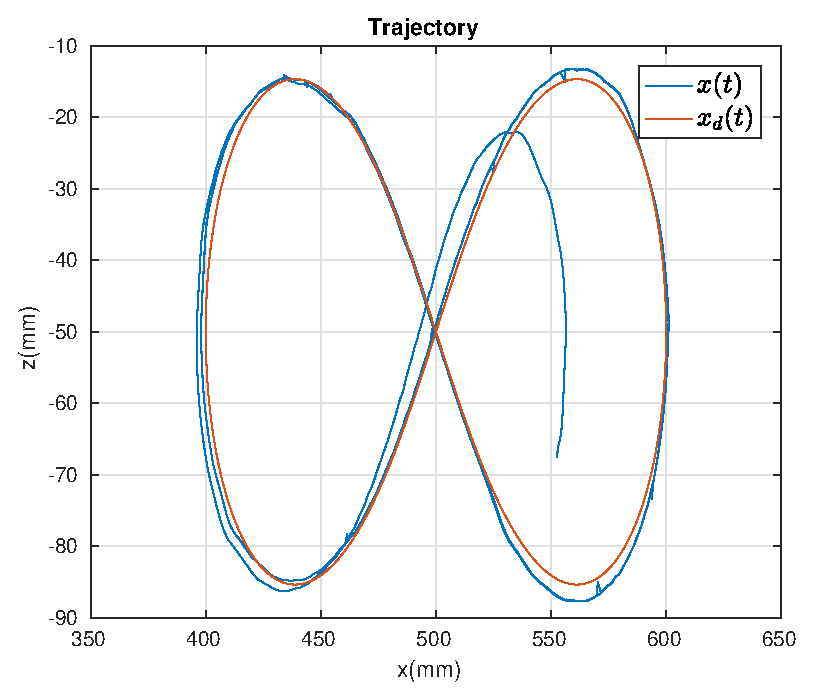
\includegraphics[width=0.5\linewidth]{./img/traj_2_k1/traj.eps}
  \caption{Trajetória 2 no plano x-z}
  \label{fig:sub1}
\end{figure}%

\begin{figure}[H]
\centering
\begin{subfigure}{.5\textwidth}
  \centering
  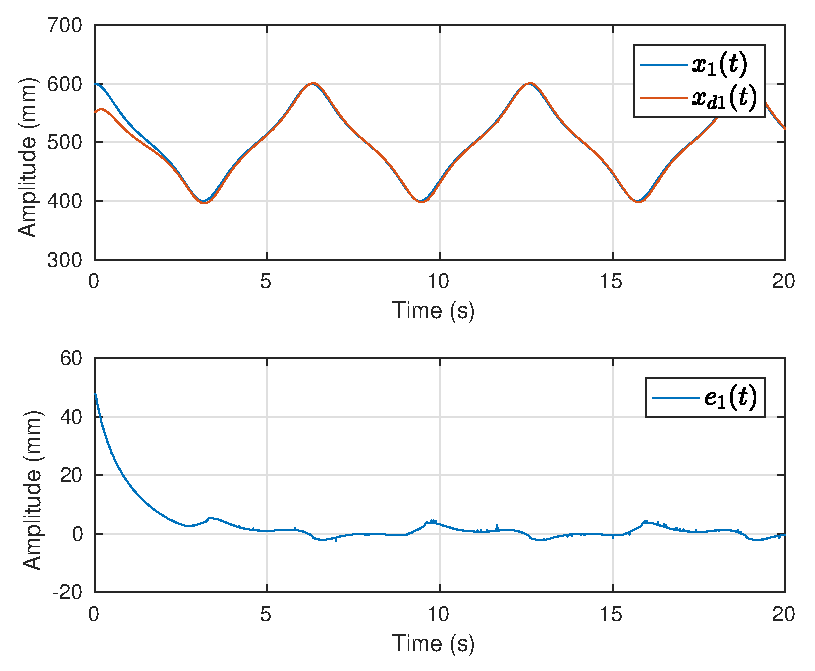
\includegraphics[width=\linewidth]{./img/traj_2_k1/x1.eps}
  \caption{$x_1$}
  \label{fig:sub1}
\end{subfigure}%
\begin{subfigure}{.5\textwidth}
  \centering
  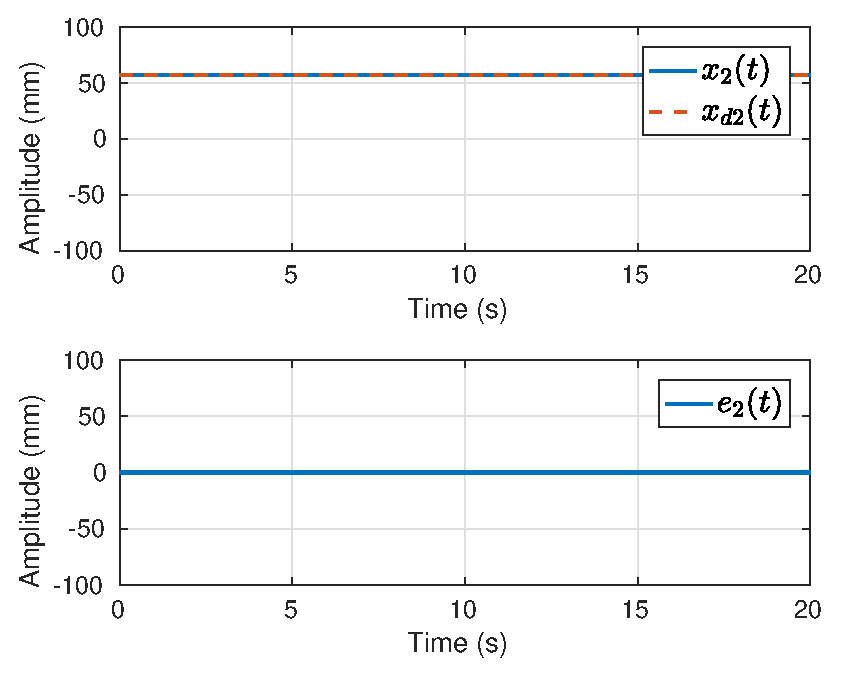
\includegraphics[width=\linewidth]{./img/traj_2_k1/x2.eps}
  \caption{$x_2$}
  \label{fig:sub2}
\end{subfigure}
\begin{subfigure}{.5\textwidth}
  \centering
  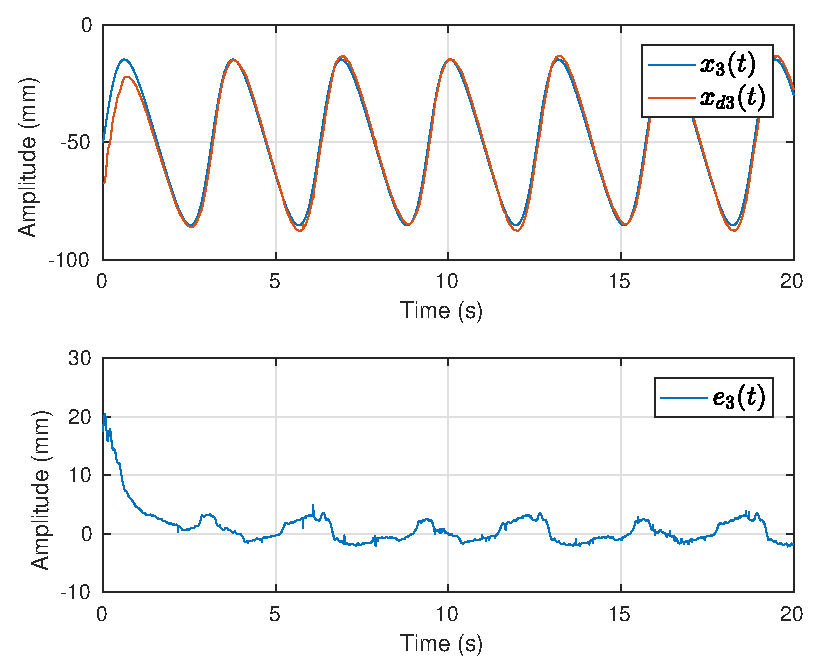
\includegraphics[width=\linewidth]{./img/traj_2_k1/x3.eps}
  \caption{$x_3$}
  \label{fig:sub1}
\end{subfigure}%
\begin{subfigure}{.5\textwidth}
  \centering
  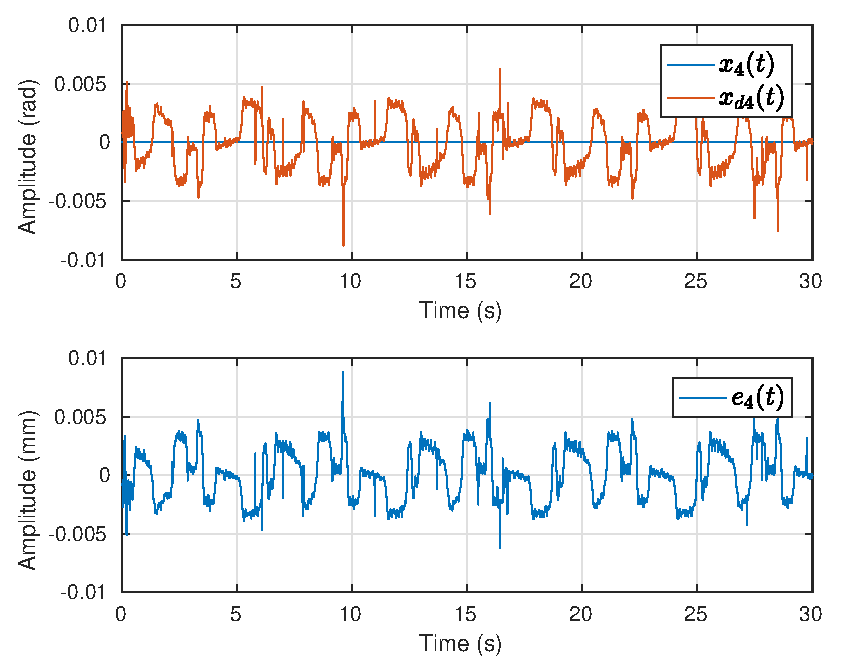
\includegraphics[width=\linewidth]{./img/traj_2_k1/x4.eps}
  \caption{$x_4$}
  \label{fig:sub2}
\end{subfigure}
\caption{Resultados experimentas - Rastreamento da trajetória 2 para $\bm{K}_t = \bm{I}$}
\label{fig:test}
\end{figure}

\begin{figure}[H]
\centering
\begin{subfigure}{.5\textwidth}
  \centering
  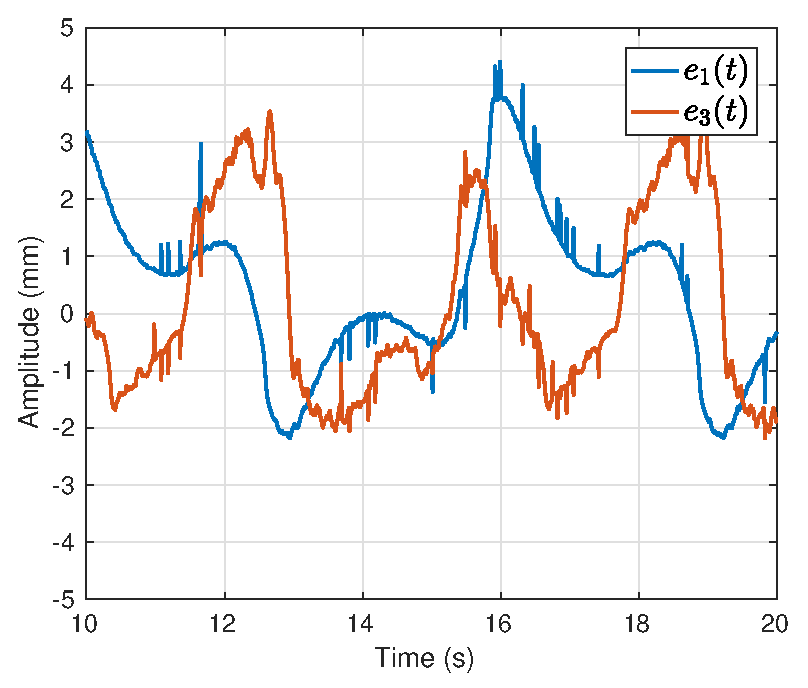
\includegraphics[width=\linewidth]{./img/traj_2_k1/error.eps}
  \caption{$e_1$}
  \label{fig:sub1}
\end{subfigure}%
\begin{subfigure}{.5\textwidth}
  \centering
  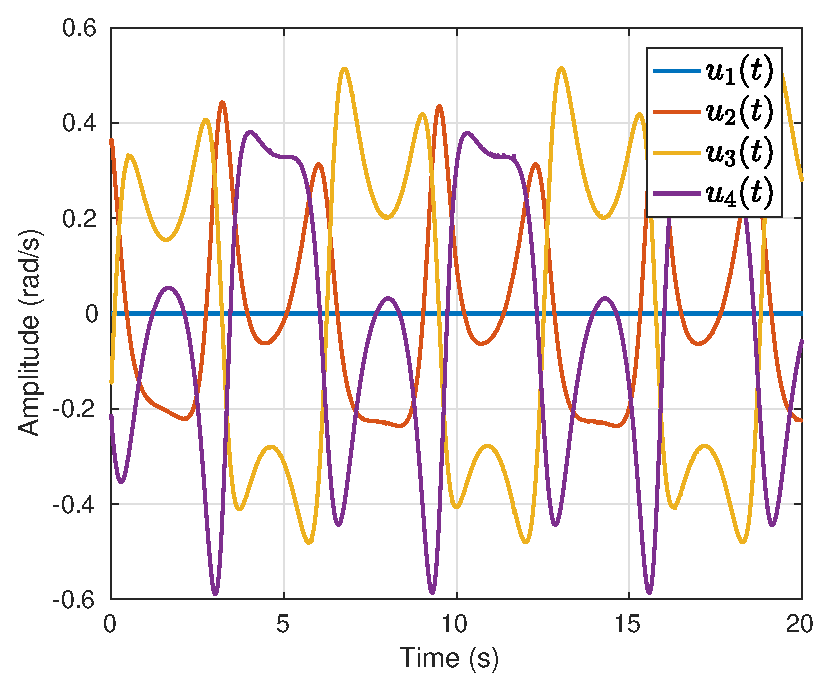
\includegraphics[width=\linewidth]{./img/traj_2_k1/u.eps}
  \caption{$e_3$}
  \label{fig:sub2}
\end{subfigure}
\caption{Resultados experimentas - Trajetória 2: Destaque para o erro $e_1$ e $e_3$ com $\bm{K}_t = \bm{I}$}
\label{fig:erro_traj}
\end{figure}

\subsubsection{Ganho $\bm{K}_t = 5\bm{I}$}

\begin{figure}[H]
\centering
  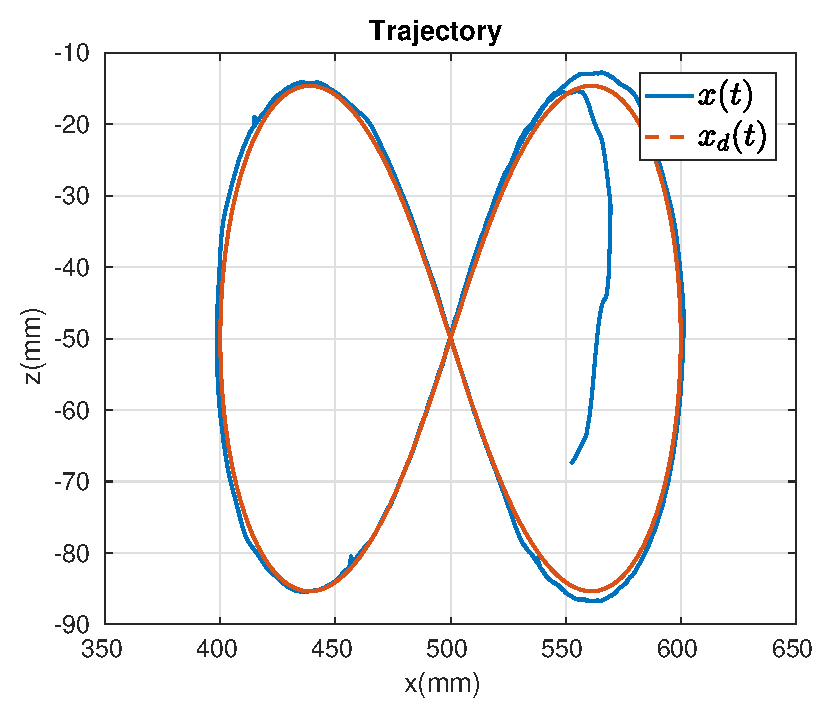
\includegraphics[width=0.5\linewidth]{./img/traj_2_k5/traj.eps}
  \caption{Resultados experimentas - Trajetória 2 no plano x-z para $\bm{K}_t = 5\bm{I}$}
  \label{fig:sub1}
\end{figure}%

\begin{figure}[H]
\centering
\begin{subfigure}{.5\textwidth}
  \centering
  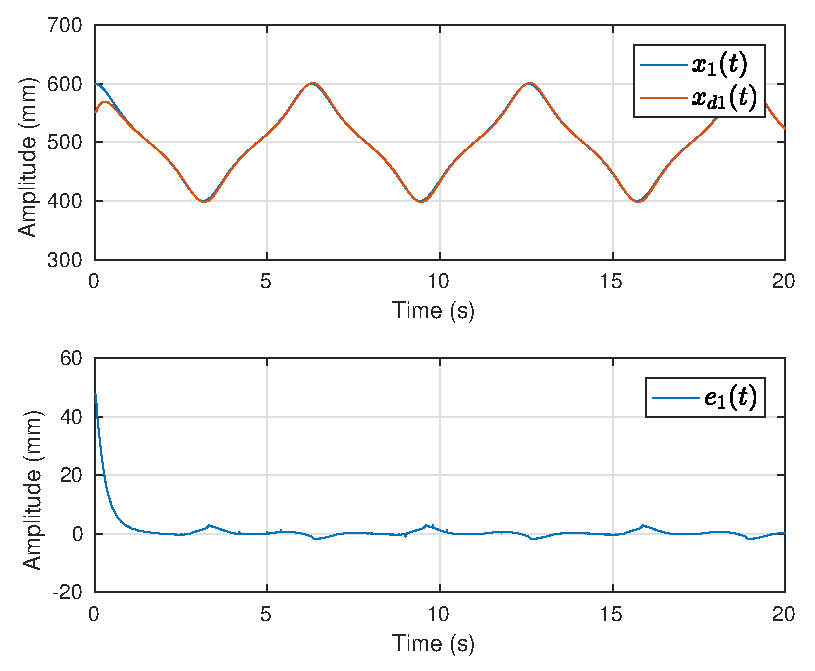
\includegraphics[width=\linewidth]{./img/traj_2_k5/x1.eps}
  \caption{$x_1$, $x_{d1}$ e $e_1$}
  \label{fig:sub1}
\end{subfigure}%
\begin{subfigure}{.5\textwidth}
  \centering
  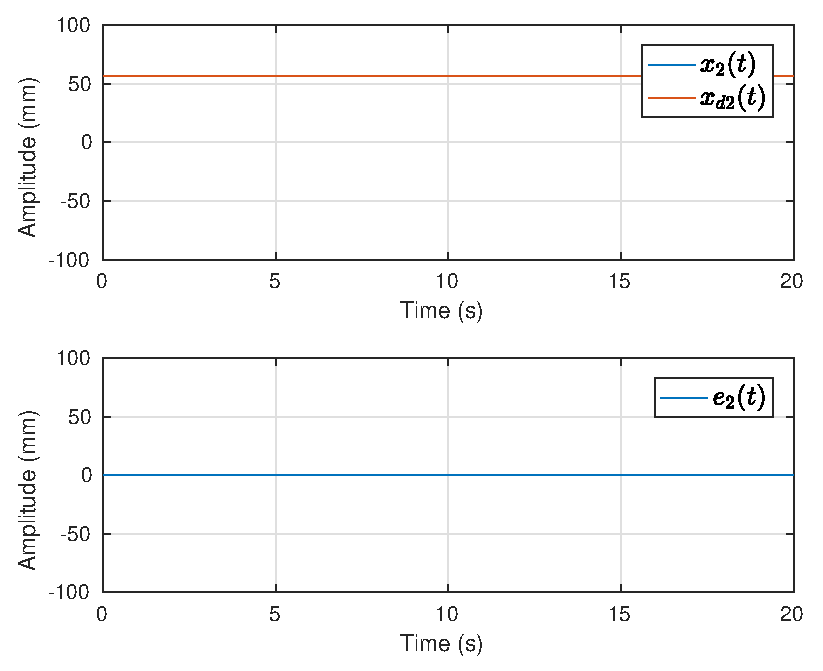
\includegraphics[width=\linewidth]{./img/traj_2_k5/x2.eps}
  \caption{$x_2$, $x_{d2}$ e $e_2$}
  \label{fig:sub2}
\end{subfigure}
\begin{subfigure}{.5\textwidth}
  \centering
  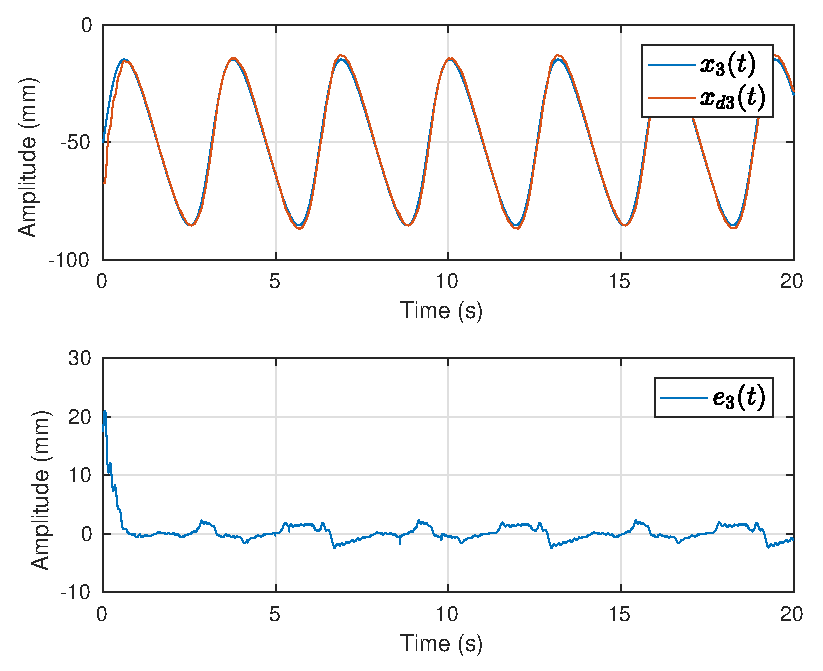
\includegraphics[width=\linewidth]{./img/traj_2_k5/x3.eps}
  \caption{$x_3$, $x_{d3}$ e $e_3$}
  \label{fig:sub1}
\end{subfigure}%
\begin{subfigure}{.5\textwidth}
  \centering
  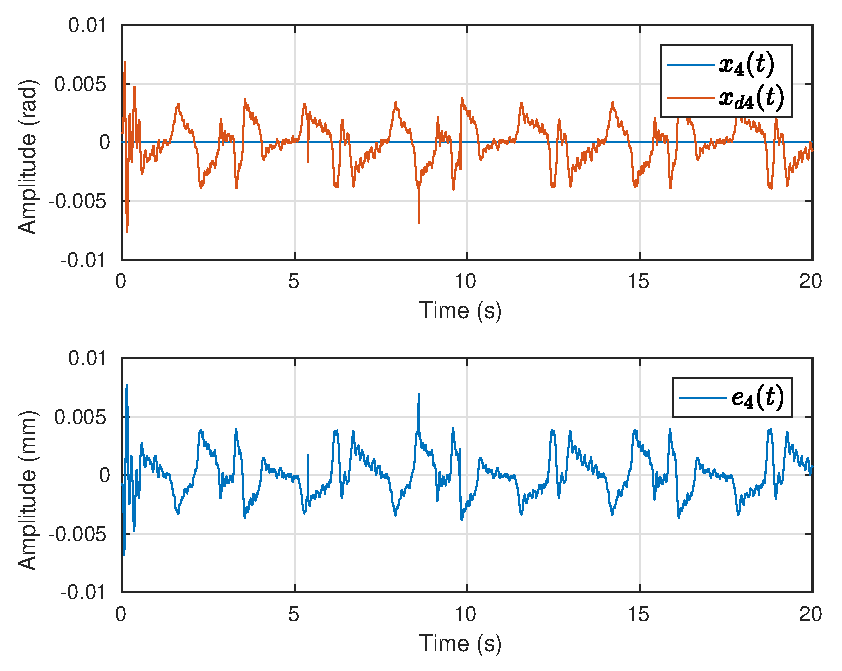
\includegraphics[width=\linewidth]{./img/traj_2_k5/x4.eps}
  \caption{$x_4$, $x_{d4}$ e $e_4$}
  \label{fig:sub2}
\end{subfigure}
\caption{Rastreamento da trajetória 2 para $\bm{K}_t = 5\bm{I}$}
\label{fig:test}
\end{figure}

\begin{figure}[H]
\centering
\begin{subfigure}{.5\textwidth}
  \centering
  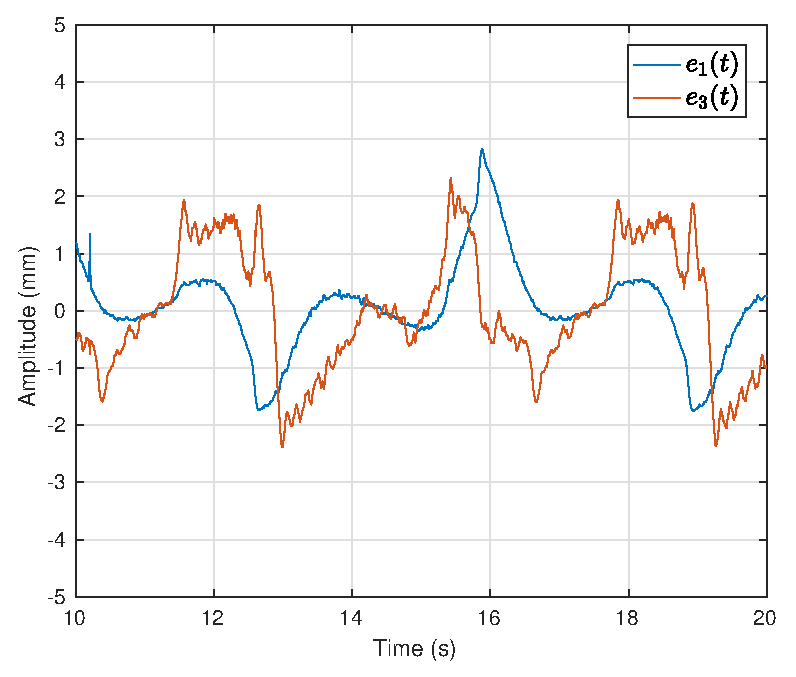
\includegraphics[width=\linewidth]{./img/traj_2_k5/error.eps}
  \caption{$e_1$}
  \label{fig:sub1}
\end{subfigure}%
\begin{subfigure}{.5\textwidth}
  \centering
  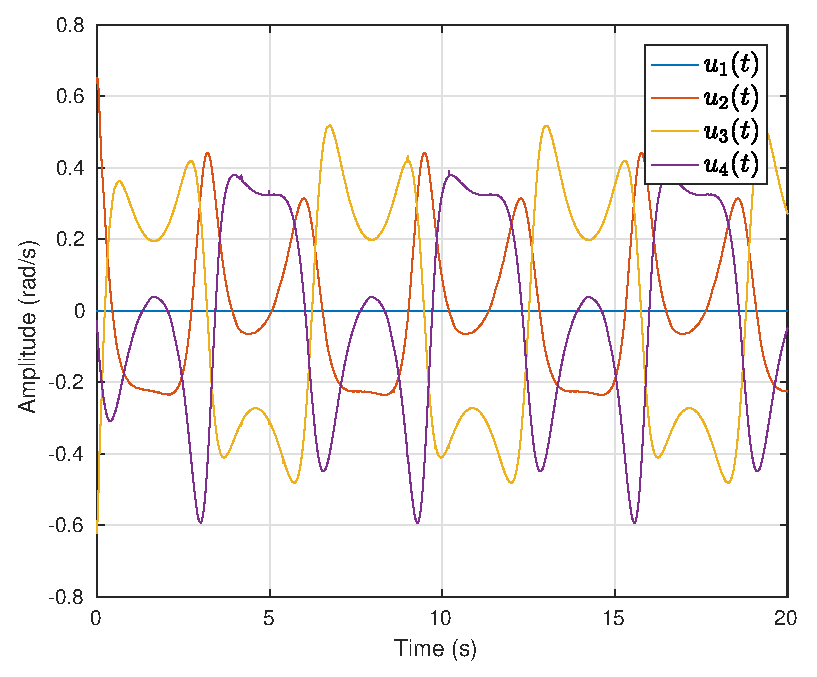
\includegraphics[width=\linewidth]{./img/traj_2_k5/u.eps}
  \caption{$e_3$}
  \label{fig:sub2}
\end{subfigure}
\caption{Trajetória 2: destaque para o erro $e_1$ e $e_3$}
\label{fig:erro_traj}
\end{figure}

A partir da variação do ganho de controle foi possível concluir que o fator principal que gera erro em regime permanente, não é 
\section{Controle de Força}

Nesta seção demonsta-se os reultados de experimentos de controle de força, segundo os estratégias definidas em \ref{sec:force}. 

\subsection{Float}
Neste experimento a referência de força é configurada para zero, logo é possível mover o efetuador aplicando forças sobre ele. O operador tentou traçar um retângulo no plano x-z.

\begin{figure}[H]
\centering
\begin{subfigure}{.5\textwidth}
  \centering
  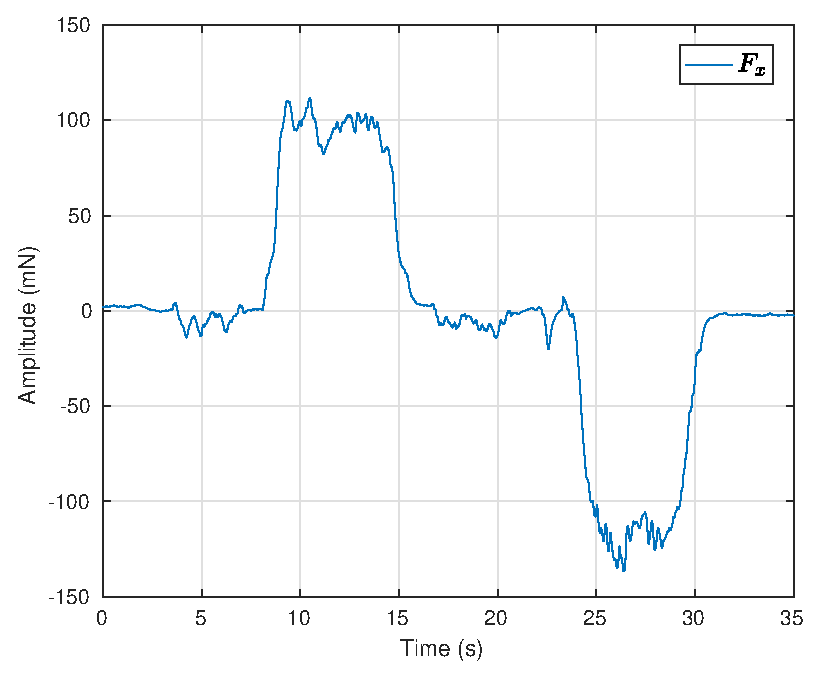
\includegraphics[width=\linewidth]{./img/float2/Fx.eps}
  \caption{$F_x$}
  \label{fig:sub1}
\end{subfigure}%
\begin{subfigure}{.5\textwidth}
  \centering
  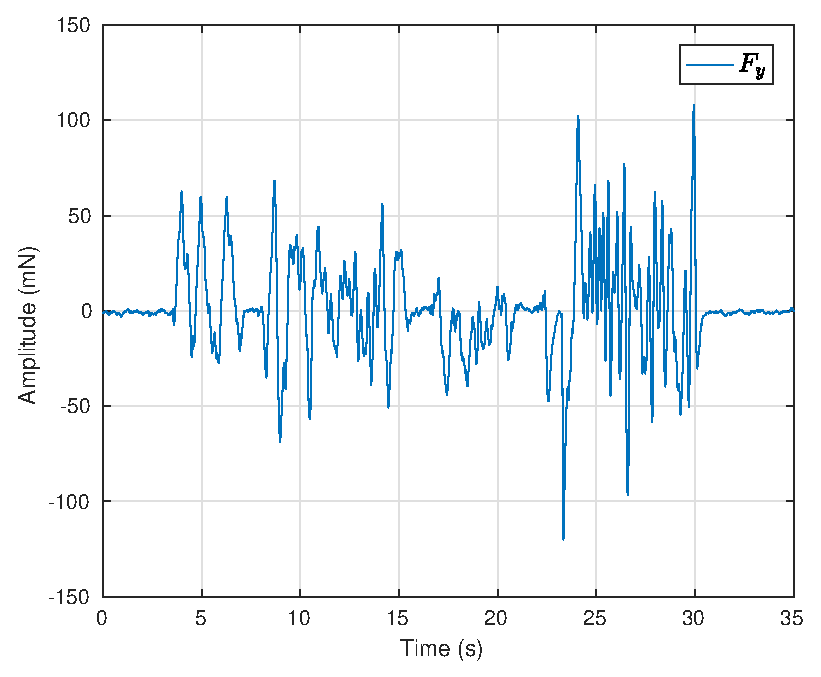
\includegraphics[width=\linewidth]{./img/float2/Fy.eps}
  \caption{$F_y$}
  \label{fig:sub2}	
\end{subfigure}
\begin{subfigure}{.5\textwidth}
  \centering
  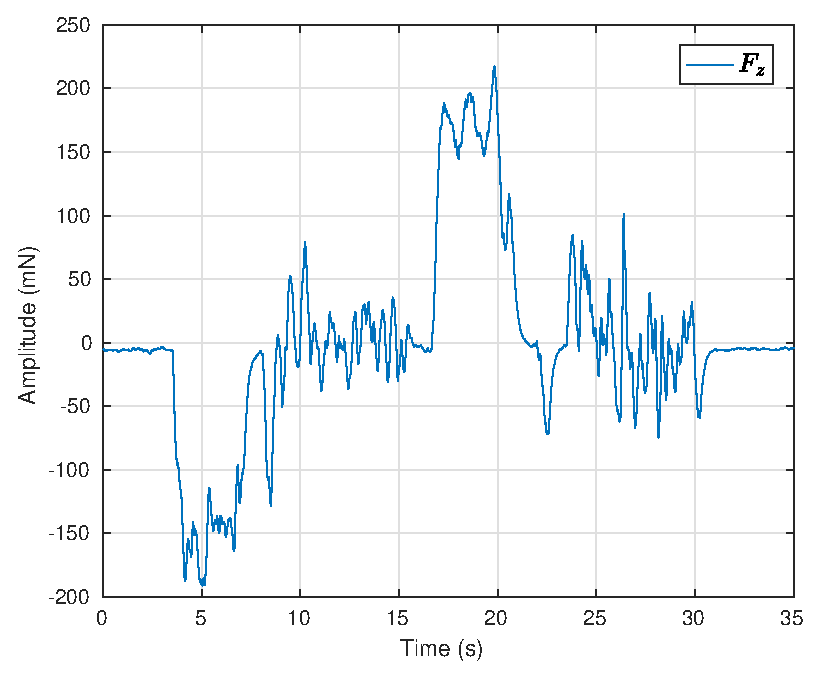
\includegraphics[width=\linewidth]{./img/float2/Fz.eps}
  \caption{$F_z$}
  \label{fig:sub1}
\end{subfigure}%
\begin{subfigure}{.5\textwidth}
  \centering
  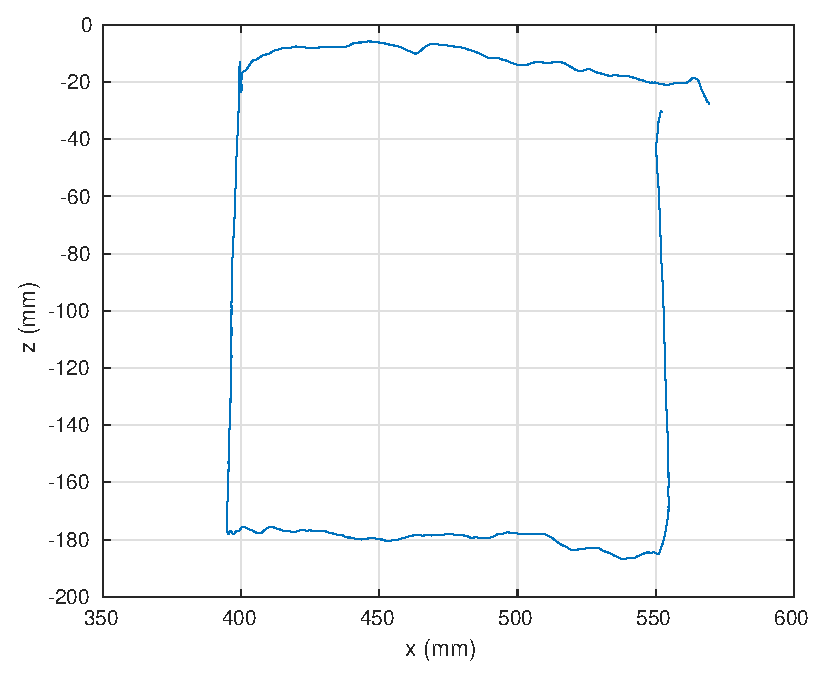
\includegraphics[width=\linewidth]{./img/float2/xz.eps}
  \caption{Plano $xz$}
  \label{fig:sub2}
\end{subfigure}
\caption{Resultados experimentais - Controle de Força: Float}
\label{fig:test}
\end{figure}

\subsection{Approach}
Considerando o problema de aplicar uma força em uma placa de poliestireno montada em um suporte fixado na vertical como mostra a figura \ref{fig:suporte_forca}.  Conforme mostrado em \ref{sec:forca_approach} a força de contato pode ser modelada pela lei de Hooke, portanto é necessário saber a constante elástica do ambiente.

Foi feito um ensaio para encontrar a constante $k_s$ variando a distância $x_s$ e medindo a força resultante. Os dados experimentais e a regressão linear pode ser vista na figura \ref{fig:ks_linreg}. A constante encontrada foi $k_s = 379.7642 N/m$.

\begin{figure}[!ht]
\centering
  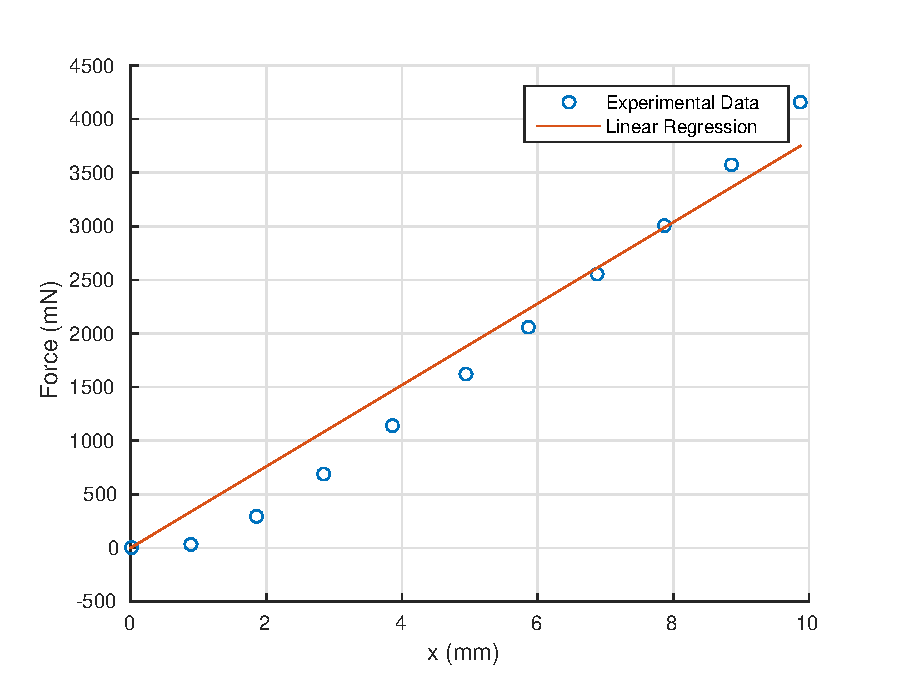
\includegraphics[width=0.5\linewidth]{./img/ks_estimation.eps}
  \caption{Estimação da constante elástica $k_s$ e regressão linear.}
  \label{fig:ks_linreg}
\end{figure}%

Foi aplicado o controle de força com uma referência constante de $1000 mN$ na direção de \textit{approach}, sobre uma placa de poliestireno utilizando ganho do controlador PI de $k_p = 2$ e $k_i = 0.05$. 

 \begin{figure}[H]
  \centering
  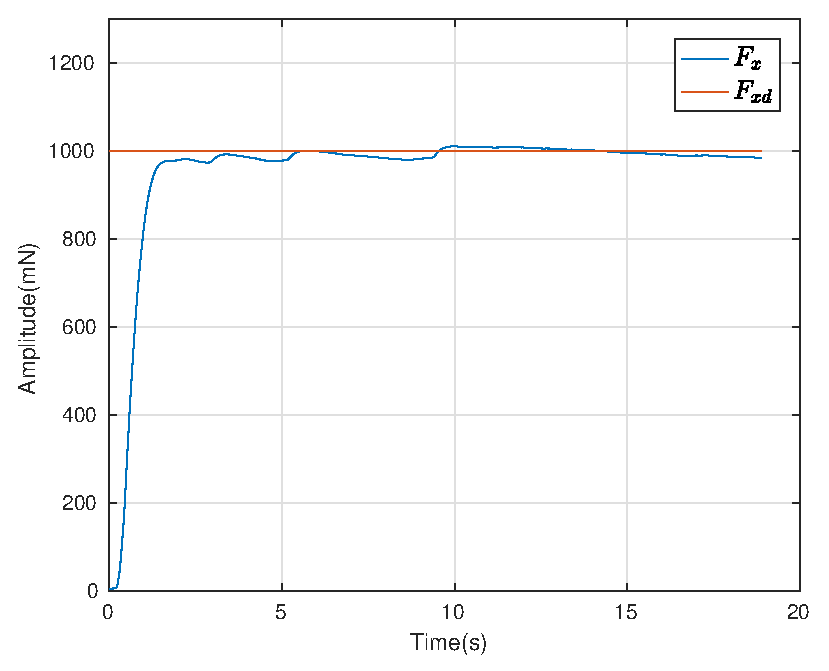
\includegraphics[width=0.5\linewidth]{./img/force1000_kp2_ki005/Fx.eps}
  \caption{Resultados experimentais - Controle de força: Approach $Fx$}
  \label{fig:sub2}
\end{figure}

Os resultados mostraram a existência de não linearidades que não foram consideradas no modelo. Por exemplo a relação entre força e distância no ambiente testado não é exatamente linear, no entanto a aproximação foi aceitável. O fato de o sensor de força ter uma alta relação sinal-ruído para a ordem de grandeza do o sinal de referência também contribuiu para os resultados não ideais mostrados. 

